\documentclass{beamer}	
\mode<presentation>
 
\usepackage{pdfpages}
\usepackage{fancyvrb}
\usepackage{chemarr}

\usepackage{amsmath}		%% mathematics typesetting
\usepackage{amssymb}
 
\usepackage{epigraph}   %% nice setting of quotations

\usepackage{tabularx} %% allows to use row colours in tables

\usepackage{ulem}

\usepackage{booktabs}

\usepackage{siunitx} %% tpyeset SI units

\usepackage{CJKutf8} %% typeset Chinese characters

\usepackage{pdfpages}%% include pdfs

\usepackage{graphicx}
\usepackage{animate} %% show animated gifs

\DeclareMathAlphabet{\mathcalligra}{T1}{calligra}{m}{n}




% Color and Theme. Can be changed. However, this one's quite nice.
\usetheme{Madrid}
\setbeamertemplate{page number in head/foot}{}

\definecolor{theme}{rgb}{0.84,0,0.21}
\usecolortheme[named=theme]{structure}


% \beamertemplatenavigationsymbolsempty

\begin{document}




%%%%%%%%%%%%%%%%%%%%%%%%%%%%%%%%%%%%%%%%%%%%%%%%%%
%%%%%%%%%%%%%%%%%%%%%%%%%%%%%%%%%%%%%%%%%%%%%%%%%%
%%%%%%%%%%%%%%%%%%%%%%%%%%%%%%%%%%%%%%%%%%%%%%%%%%



\begin{frame}{M11.10 Hormone und Regelkreise}
%% Hormone

%% Einteilung von Hormonen: Chemische Eigenschaften, Wirkungsort, Gewebe der Bildung, Wirkungsweise
%% Regelkreise

\begin{columns}[c]

\begin{column}{5cm}

\begin{block}{nach Chemie}

 \textbf{Peptid/Aminosäurederivate}: \\
 Wasserlöslich (außer T3/T4) \\
 Wirken über metabotrope Rezeptoren in der Zellmembran  \\
 Wirken schnell
 
\textbf{Steroidhormone}: \\
Fettlöslich \\
Brauchen Transportproteine \\
Wirken im Inneren der Zelle \\
Wirken langsam \\


\end{block}

\begin{block}{nach Wirkungsort}
Nach Wirkungsort: parakrin, autokrin, endokrin
\end{block}



\end{column}


\begin{column}{6cm}

\begin{block}{nach Bildungsort}
Glanduläre Hormone (Drüse) \\
Gewebshormone
\end{block}

\pause

\textbf{(Hormoneller) Regelkreis}

\begin{center}
    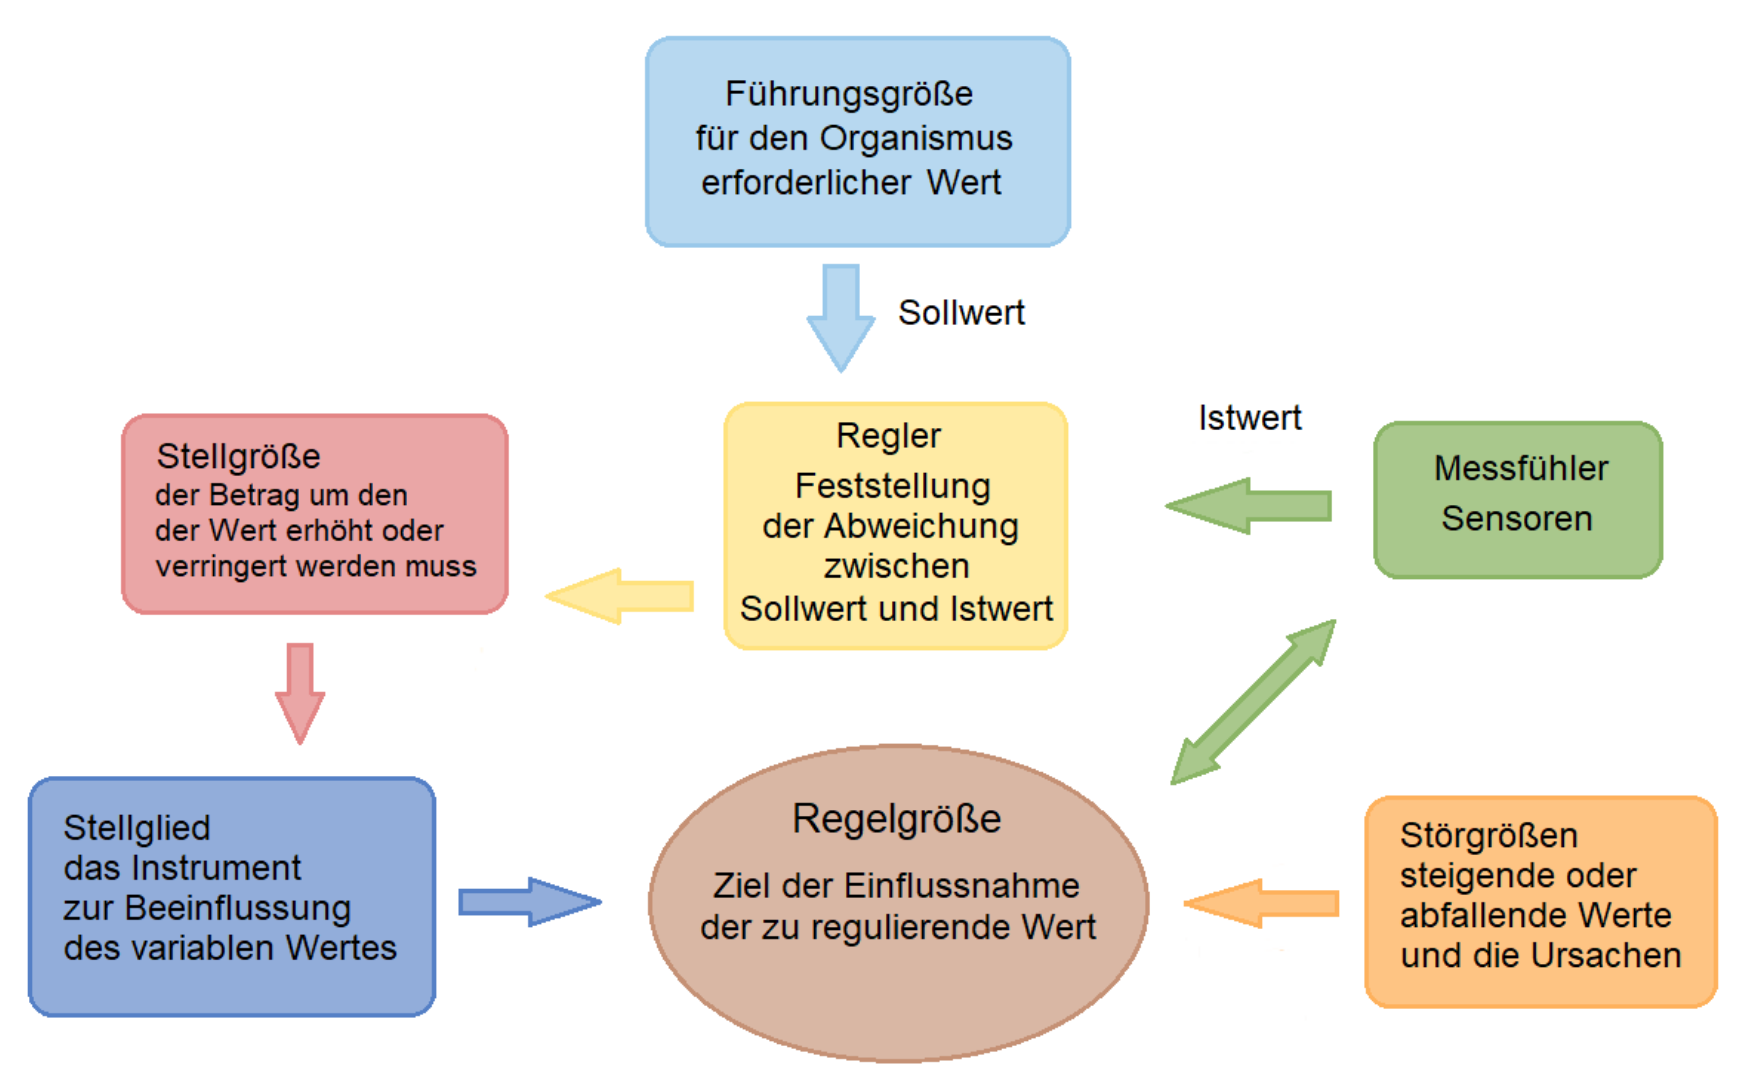
\includegraphics[width=1.1\textwidth]{regelkreis.png}
\end{center}

\end{column}


\end{columns}

    
\end{frame}


%% Hypothalamus Hypophyse allgemein
\begin{frame}{M11.10 Hormone und Regelkreise}
\begin{center}
    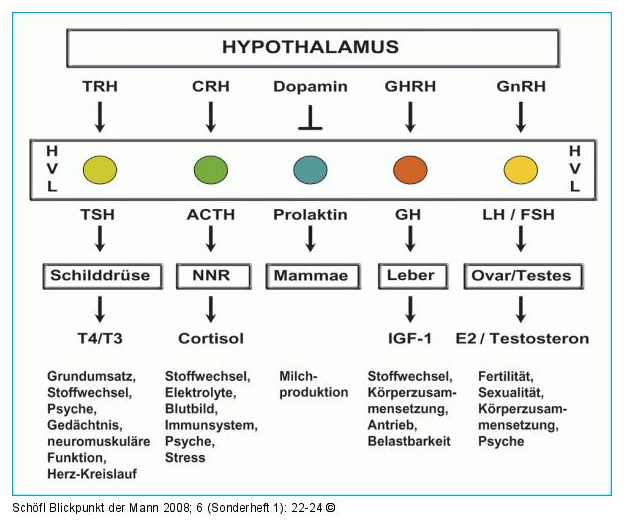
\includegraphics[width=0.7\textwidth]{hypothalamus_hypophyse.png}
\end{center}

+ Symptome bei Überschuss und bei verringerter Ausschüttung

\end{frame}




%% Thyreotropin releasong hormone: 321
\begin{frame}{IMPP Fragen}
\textbf{
Thyreotropin-Releasing-Hormon (TRH)} \\[0.2 cm]

\begin{itemize}
\item[A.] hemmt die Freisetzung der Schilddrüsenhormone T\textsubscript{3} und T\textsubscript{4}
\item[B.] ist ein dimeres Proteohormon
\item[C.] stimuliert die Freisetzung des Thyreoidea-stimulierenden Hormons (TSH) %% correct
\item[D.] wird extra-ribosomal ATP-abhängig synthetisiert
\item[E.] wird hauptsächlich durch hepatische Konjugation inaktiviert 

\end{itemize}
    
\end{frame}

\begin{frame}{IMPP Fragen}
\textbf{
Thyreotropin-\textcolor{blue}{Releasing}-Hormon (TRH)} \\[0.2 cm]

\begin{itemize}
\item[A.] hemmt die Freisetzung der Schilddrüsenhormone T\textsubscript{3} und T\textsubscript{4}
\item[B.] ist ein dimeres Proteohormon
\item[C.] \textcolor{blue}{stimuliert die Freisetzung des Thyreoidea-stimulierenden Hormons (TSH)} %% correct
\item[D.] wird extra-ribosomal ATP-abhängig synthetisiert
\item[E.] wird hauptsächlich durch hepatische Konjugation inaktiviert 

\end{itemize}
    
\end{frame}






%% Cushing Syndrom: 171
\begin{frame}{IMPP Fragen}

\textbf{Bei einer Patientin treten folgende Störungen gemeinsam auf: arterieller Bluthochdruck, Hyperglykämie, stammbetonte Adipositas bei Verringerung der Muskelmasse an den Extremitäten.}

\textbf{Ein primärer Überschuss an welchem der folgenden Hormone kommt als Ursache der genannten Störungen am ehesten in Frage?} \\[0.2 cm]

\begin{itemize}
\item[A.] Aldosteron
\item[B.] Cortisol %% correct
\item[C.] Insulin
\item[D.] Somatotropin
\item[E.] Thyroxin

\end{itemize}
    
\end{frame}


\begin{frame}{IMPP Fragen}

\dots arterieller Bluthochdruck, \textcolor{blue}{\textbf{Hyperglykämie}}, \textcolor{blue}{\textbf{stammbetonte Adipositas}} bei Verringerung der Muskelmasse an den Extremitäten \dots

Ein primärer \textcolor{blue}{\textbf{Überschuss}} an welchem der folgenden Hormone kommt als Ursache der genannten Störungen am ehesten in Frage? \\[0.2 cm]


\begin{columns}[t]
\begin{column}{3cm}
\begin{itemize}
\item[A.] Aldosteron
\item[B.] \textcolor{blue}{Cortisol} %% correct
\item[C.] Insulin
\item[D.] Somatotropin
\item[E.] Thyroxin

\end{itemize}

\end{column}


\begin{column}{7cm}

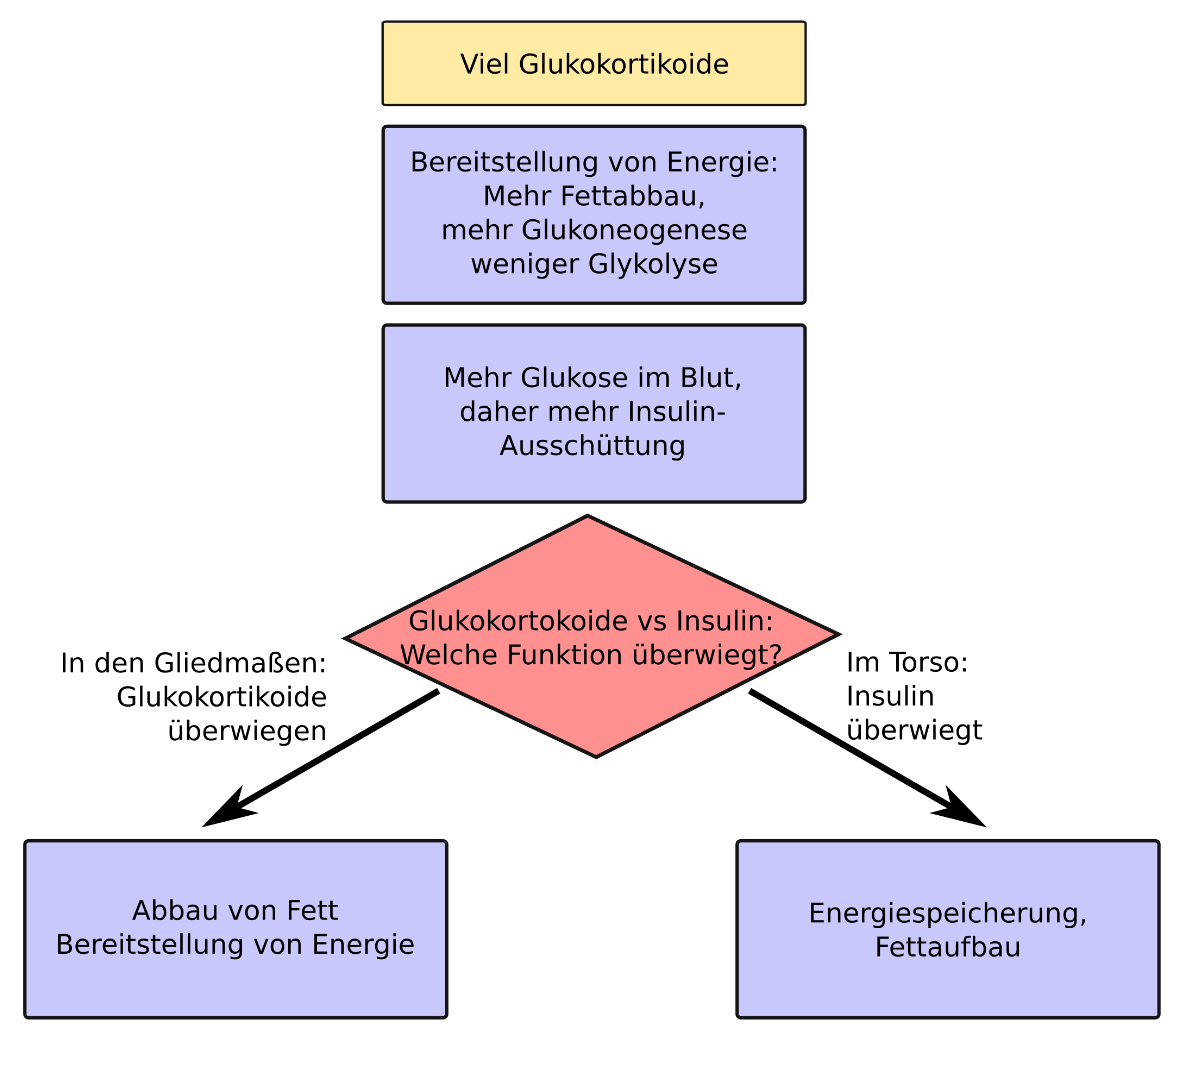
\includegraphics[width=0.9\textwidth]{glukokortikoid_ueberschuss.png}

\end{column}


\end{columns}
    
\end{frame}





%%%%%%%%%%%%%%%%%%%%%%%%%%%%%%%%%%%%%%%%%%%%%%%%%%
%%%%%%%%%%%%%%%%%%%%%%%%%%%%%%%%%%%%%%%%%%%%%%%%%%
%%%%%%%%%%%%%%%%%%%%%%%%%%%%%%%%%%%%%%%%%%%%%%%%%%


% Sexualentwicklung und Reproduktionsphysiologie I:

%% Geschlechtsspezifische Hormone: Chemie, GnRH, LH/FSH, Progesteron/Testosteron/Östrogen
%% Frühe Sexualentwicklung

\begin{frame}{M11.10 Sexualentwicklung und Reproduktionsphysiologie I}

\begin{columns}[c]

\begin{column}{5cm}

\begin{center}
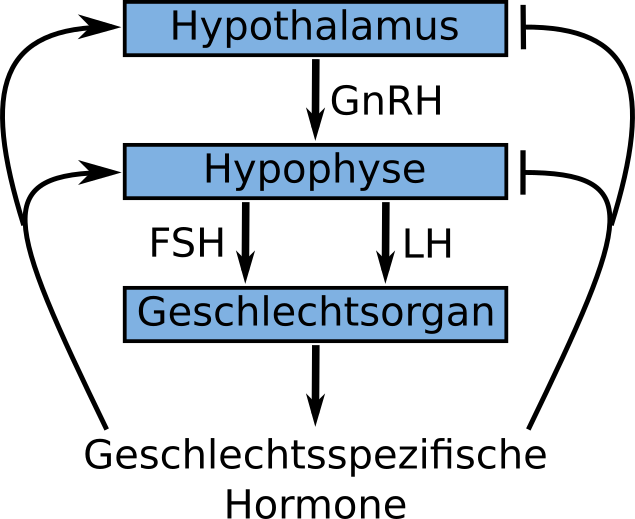
\includegraphics[width=0.7\textwidth]{geschlechtshormone_achse.png}
\end{center}

\pause

\begin{center}
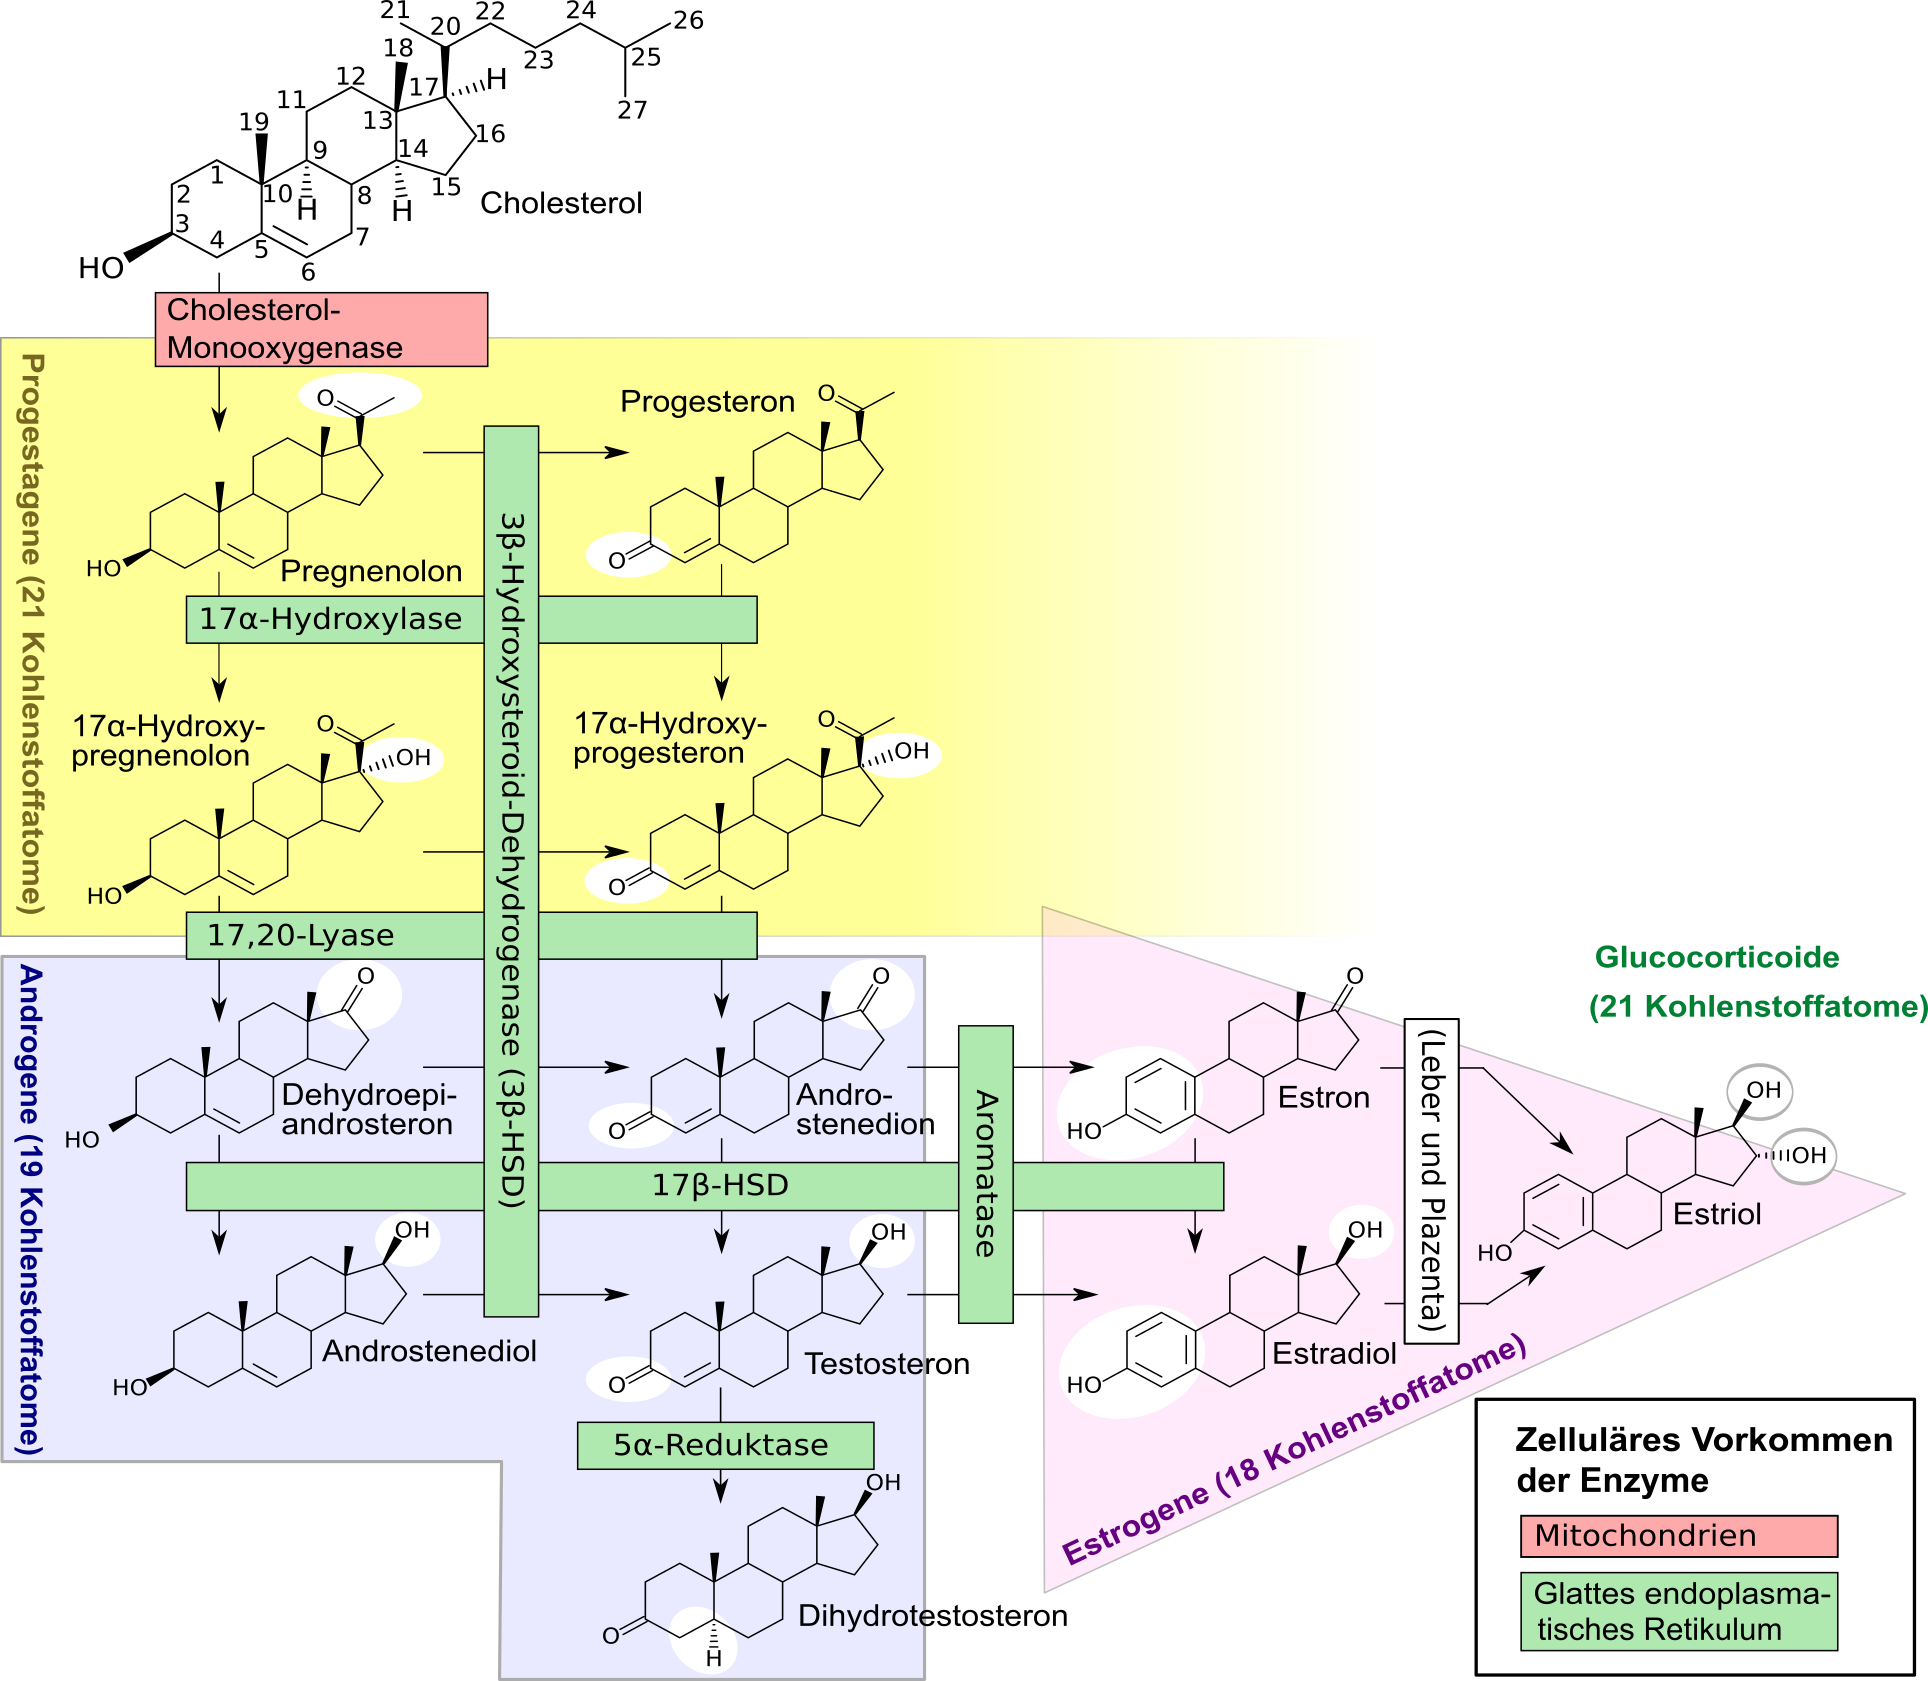
\includegraphics[width=\textwidth]{biosynthese_sexualhormone.png}
\end{center}



\end{column}

\pause

\begin{column}{6cm}

\pause

\begin{center}
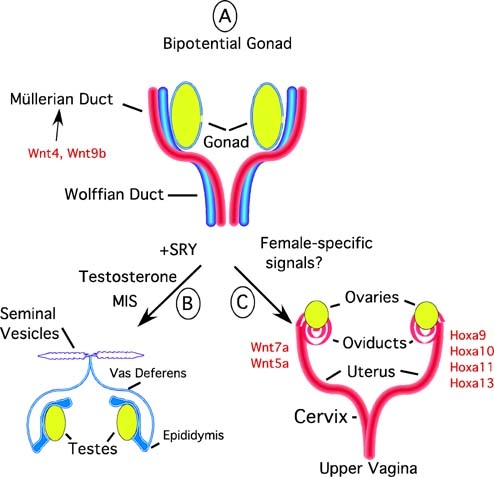
\includegraphics[width=\textwidth]{gonad_differentiation.jpg}
\end{center}


\end{column}



\end{columns}

    
\end{frame}


%5 Spermienbildung, Menstruation
\begin{frame}{M11.10 Sexualentwicklung und Reproduktionsphysiologie I}

\begin{columns}[t]

\begin{column}{5cm}

\textbf{Spermienbildung}

\begin{center}
        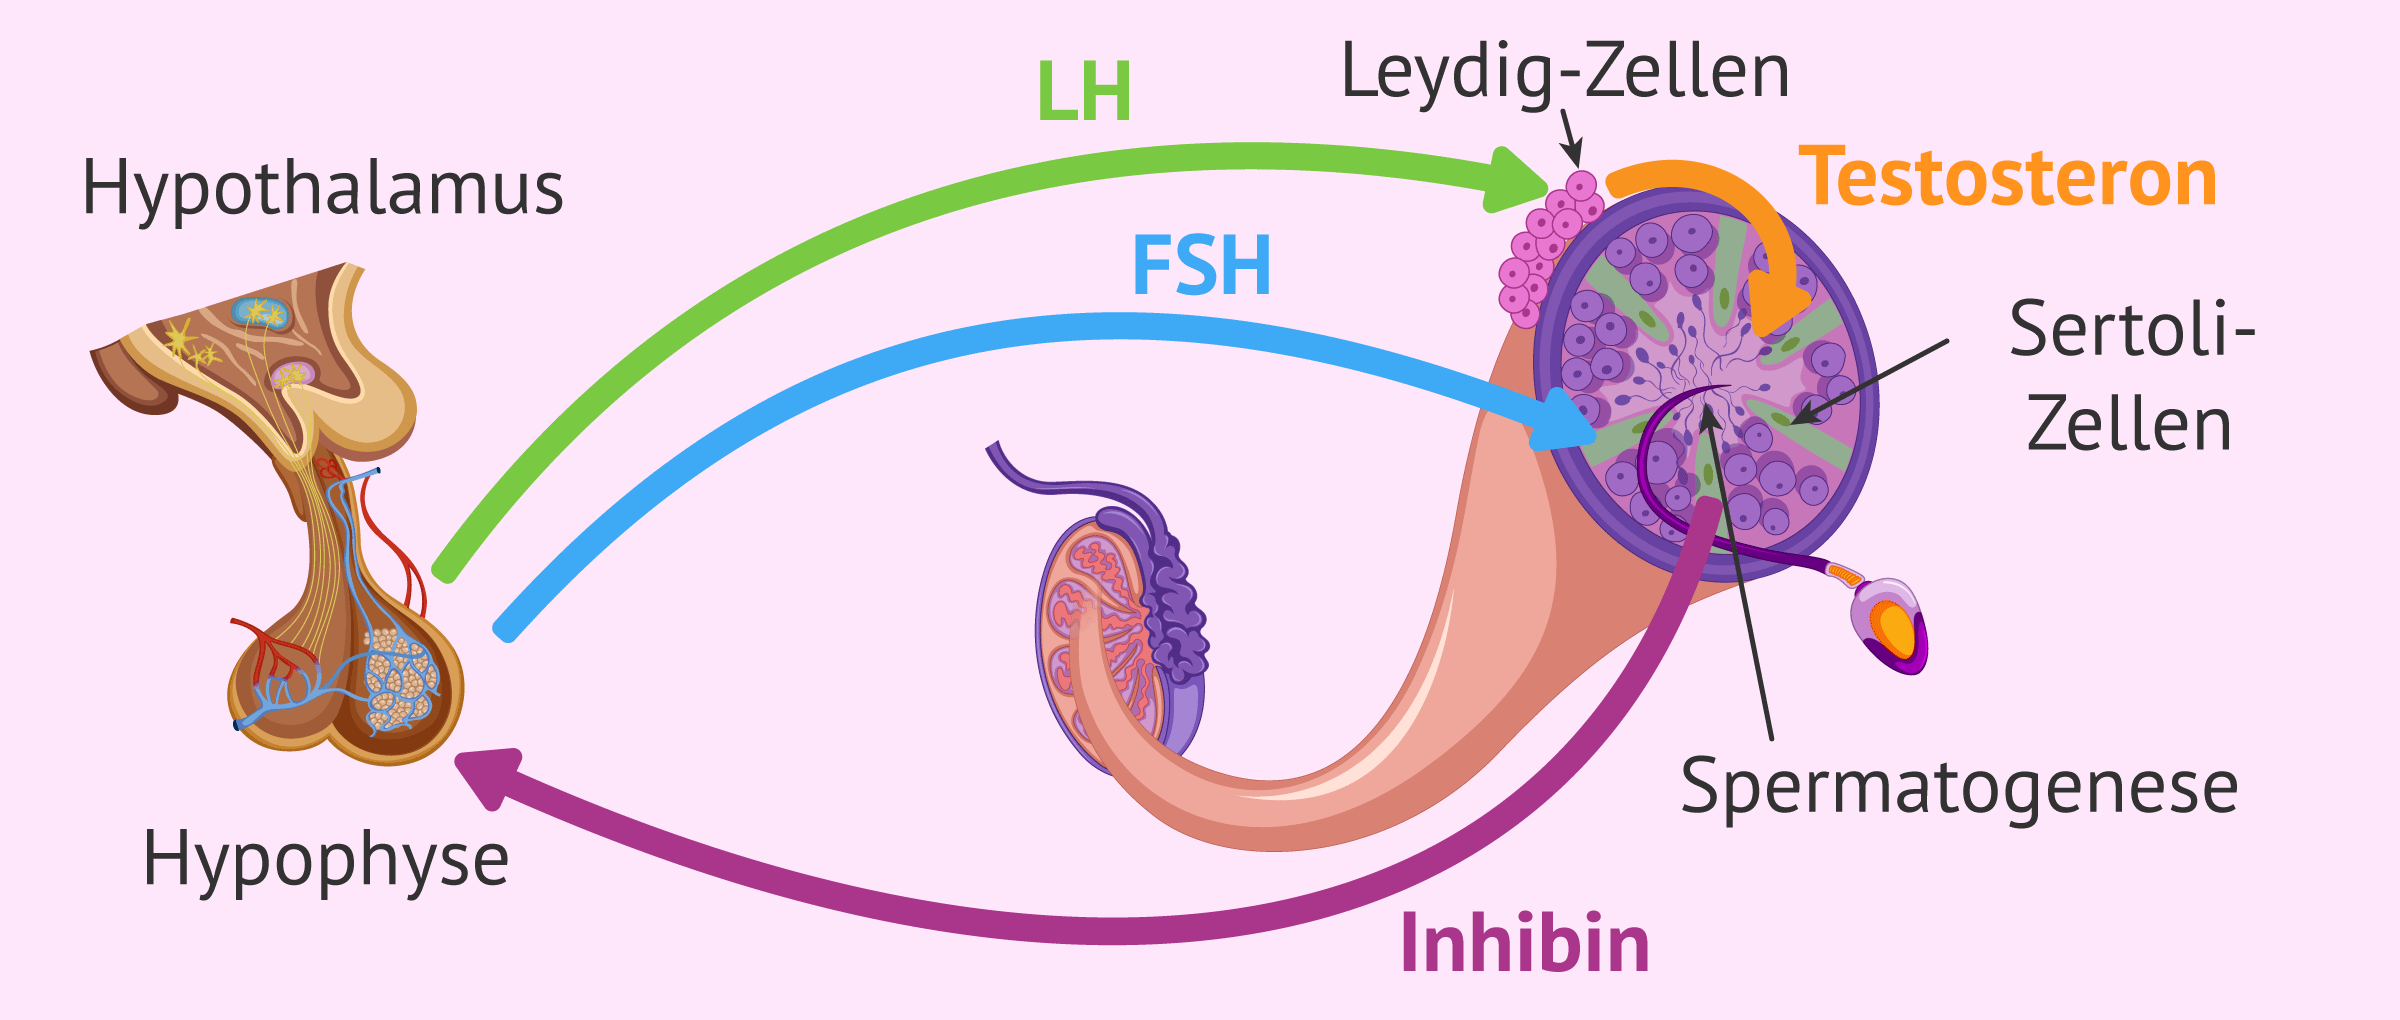
\includegraphics[width=\textwidth]{hormonelle-regulierung-spermatogenese.png}


    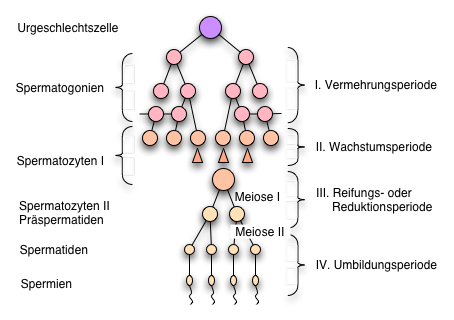
\includegraphics[width=\textwidth]{Spermatogenese.png}
    
\end{center}



\end{column}

\pause

\begin{column}{5cm}
\textbf{Menstruationszyklus}

%% Zyklus
\begin{center}
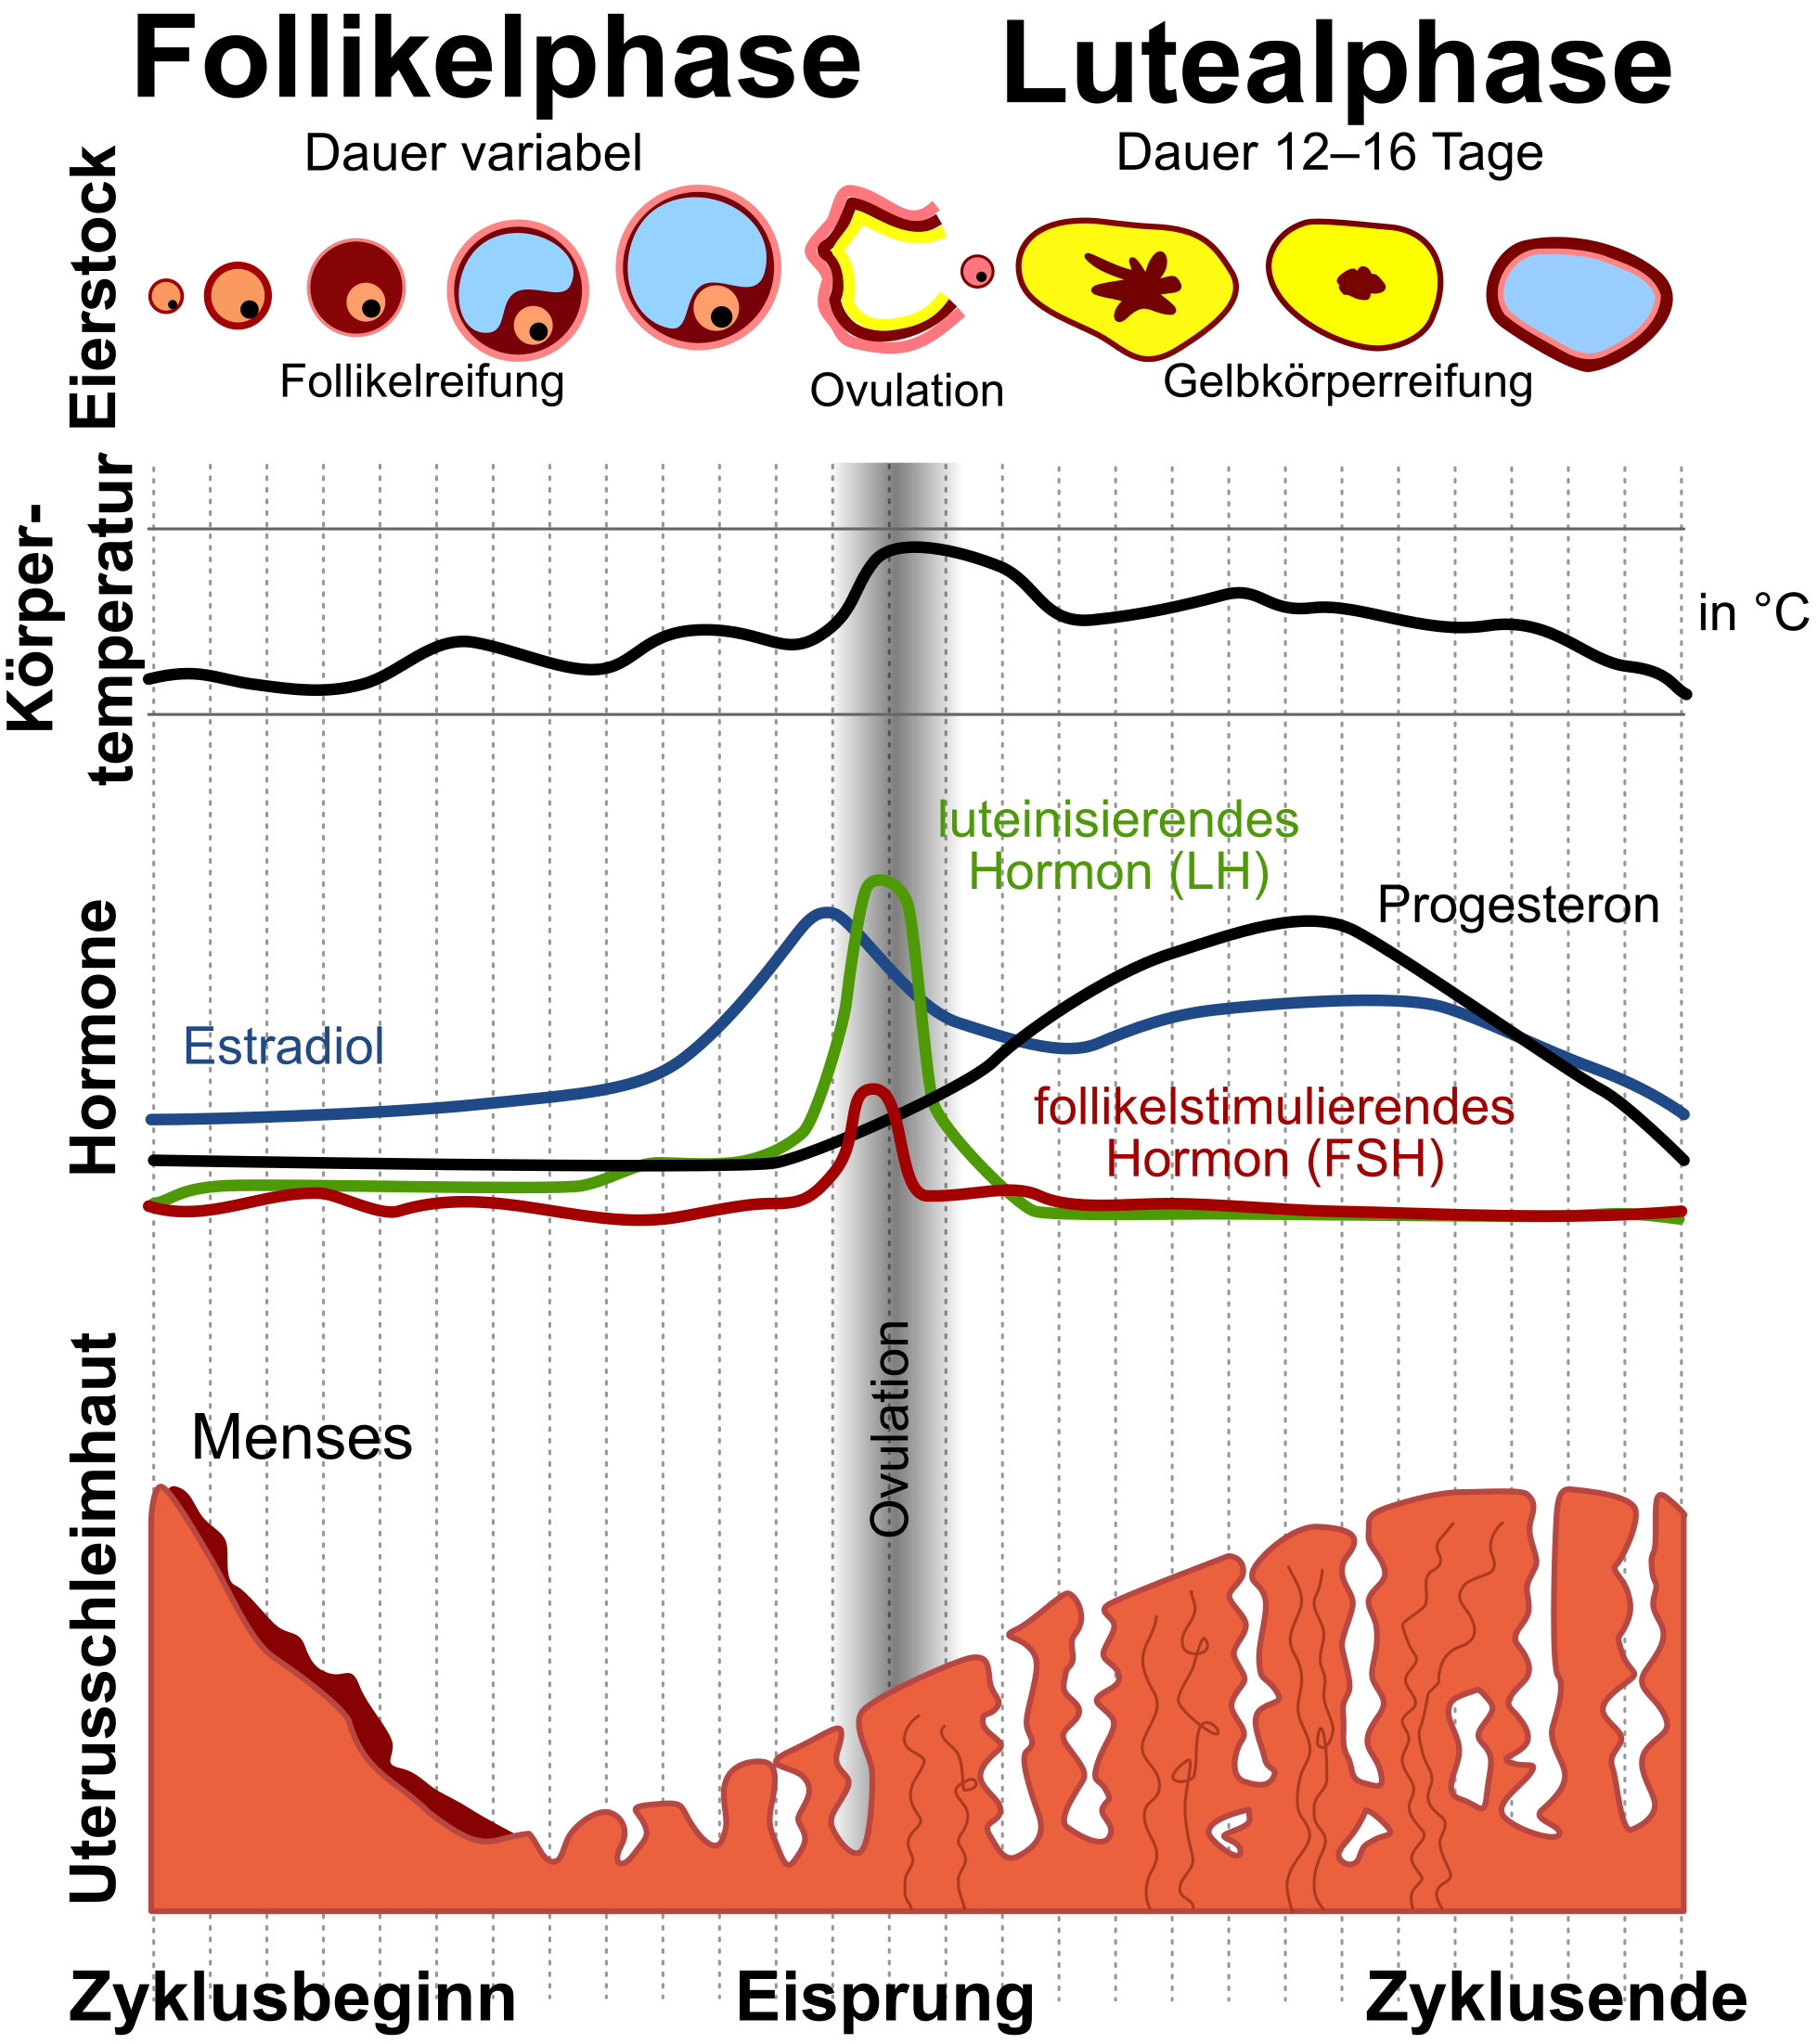
\includegraphics[width=\textwidth]{zyklus.png}
\end{center}


\end{column}


\end{columns}

\end{frame}


%% Pubertät allgemein: 

% Testosteron 281
\begin{frame}{IMPP Fragen}
    
\textbf{Welche Aussage zum Testosteron trifft typischerweise zu?} \\[0.2 cm]

\begin{itemize}
\item[A.] Testosteron wird bei männlichen Individuen erstmals in der Pubertät produziert.
\item[B.] Bei Männern stimuliert Testosteron die Sekretion von Gonadoliberin (GnRH) im Hypothalamus.
\item[C.] Bei Männern wird die Testosteron-Synthese im Hoden durch LH (Luteinisierendes Hormon) erhöht. %% correct 
\item[D.] Bei Frauen wird Testosteron im Ovar zu Progesteron umgewandelt.
\item[E.] Bei Frauen wirkt Testosteron katabol.

\end{itemize}

\end{frame}


\begin{frame}{IMPP Fragen}
    
\textbf{Welche Aussage zum Testosteron trifft typischerweise zu?} \\[0.2 cm]

\begin{itemize}
\item[A.] Testosteron wird bei männlichen Individuen erstmals in der Pubertät produziert.
\item[B.] Bei Männern stimuliert Testosteron die Sekretion von Gonadoliberin (GnRH) im Hypothalamus.
\item[C.] \textcolor{blue}{Bei Männern wird die Testosteron-Synthese im Hoden durch LH (Luteinisierendes Hormon) erhöht.} %% correct 
\item[D.] Bei Frauen wird Testosteron im Ovar zu Progesteron umgewandelt.
\item[E.] Bei Frauen wirkt Testosteron katabol.

\end{itemize}

\end{frame}

% Menstruation: 199


\begin{frame}{IMPP Fragen}
    
\textbf{Welche Aussage zur Menstruation trifft zu?} \\[0.2 cm]

\begin{itemize}
\item[A.] Der erste Tag des Menstruationszyklus ist definitionsgemäß der letzte Tag der Regelblutung.
\item[B.] Der physiologische Blutverlust im Verlauf einer Regelblutung beträgt \(250-300\,mL\).
\item[C.] Die Regelblutung geht der ischämischen Phase der Uterusschleimhaut unmittelbar voraus. 
\item[D.] Plasmin ist mitverantwortlich dafür, dass Menstruationsblut im Uteruslumen nicht als ein Thrombus vorliegt. %% correct
\item[E.] Während der Regelblutung wird das Stratum basale (sog. "Basalis") der Uterusschleimhaut vollständig abgestoßen.

\end{itemize}

\end{frame}


\begin{frame}{IMPP Fragen}
    
\textbf{Welche Aussage zur Menstruation trifft zu?} \\[0.2 cm]

\begin{itemize}
\item[A.] Der erste Tag des Menstruationszyklus ist definitionsgemäß der letzte Tag der Regelblutung.
\item[B.] Der physiologische Blutverlust im Verlauf einer Regelblutung beträgt \(250-300\,mL\).
\item[C.] Die Regelblutung geht der ischämischen Phase der Uterusschleimhaut unmittelbar voraus. 
\item[D.] \textcolor{blue}{Plasmin ist mitverantwortlich dafür, dass Menstruationsblut im Uteruslumen nicht als ein Thrombus vorliegt.} %% correct
\item[E.] Während der Regelblutung wird das Stratum basale (sog. "Basalis") der Uterusschleimhaut vollständig abgestoßen.

\end{itemize}

\end{frame}



%%%%%%%%%%%%%%%%%%%%%%%%%%%%%%%%%%%%%%%%%%%%%%%%%%
%%%%%%%%%%%%%%%%%%%%%%%%%%%%%%%%%%%%%%%%%%%%%%%%%%
%%%%%%%%%%%%%%%%%%%%%%%%%%%%%%%%%%%%%%%%%%%%%%%%%%




% Hormonelle Veränderungen im Verlauf der Schwangerschaftbeschreiben und erklären
% die Entwicklung des Embryos und Fötus erklären
% die ”Fetoplazentare Einheit” und Funktion der Plazenta erläutern
% den Geburtsvorgang beschreiben und erklären
% die hormonelle Steuerung der Laktation erklären
% Erklären, wie ein Schwangerschaftstest funktioniert
% häufige Beschwerden und Komplikationen in der Schwangerschaft erklären


%% Verlauf von Schwangerschaft und Embryonalentwicklung
\begin{frame}{M11.10 Sexualentwicklung \& Reproduktionsphysiologie II: Schwangerschaft}

\begin{columns}[c]

\begin{column}{5cm}

\begin{center}
    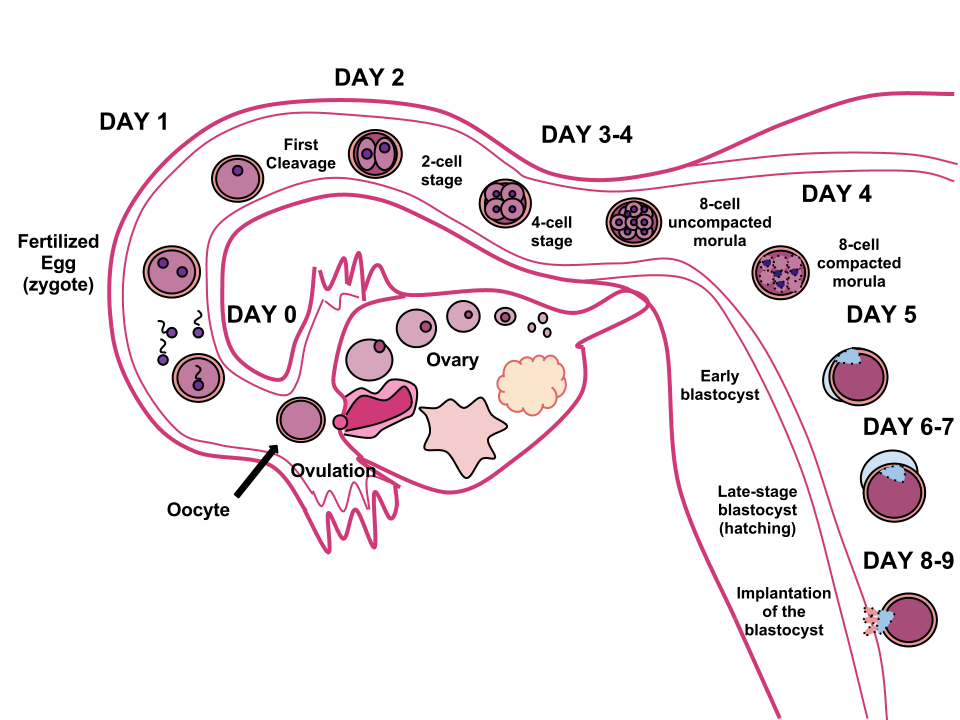
\includegraphics[width=\textwidth]{Human_Fertilization.png}
\end{center}

%% Hormone: HCG etc.
Embryo produziert humanes Choriongonadotropin (hCG). Ähnlich wie LH; fördert Progesteronbildung im Corpus luteum gravitas: Erhalt der Schwangerschaft 
\end{column}

\pause

\begin{column}{5cm}


\begin{center}
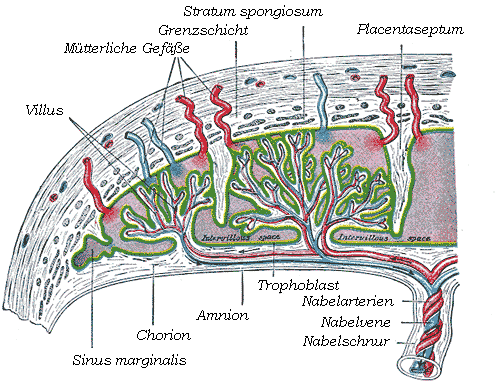
\includegraphics[width=0.8\textwidth]{Plazenta.png}    
\end{center}

% \small{Produktion von Östrogen und Progesteron ab SSW 9.}


\begin{center}
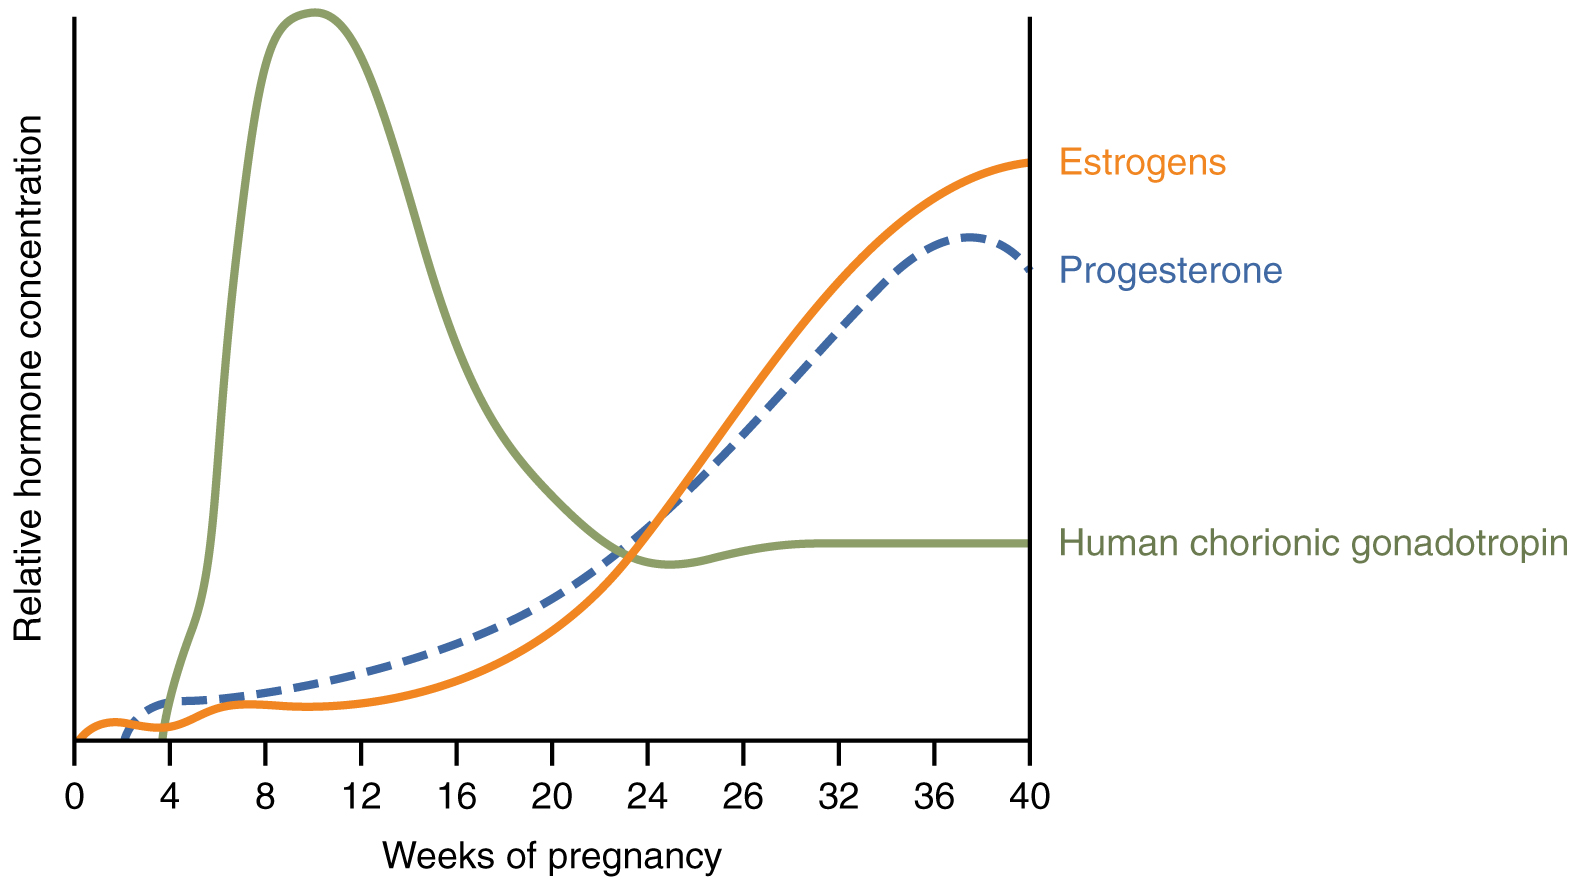
\includegraphics[width=\textwidth]{pregnancy_hormones.png}    
\end{center}



\end{column}

\end{columns}


\end{frame} 

\begin{frame}{M11.10 Sexualentwicklung \& Reproduktionsphysiologie II: Schwangerschaft}
    
    \begin{center}
        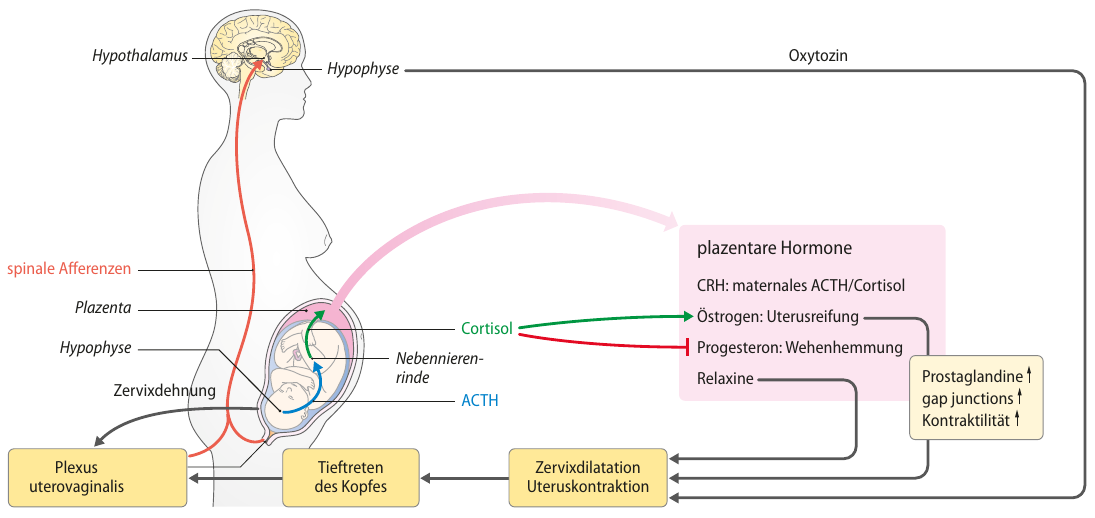
\includegraphics[width=\textwidth]{geburt_hormone.png}
    \end{center}
    
    \pause
    
    Laktation wird gesteuert durch Prolaktin aus der Adenohypophyse (Milchbildung) und Oxytocin aus der Neurohypophyse (Milchfluss). Positive Rückkopplung durch Mechanorezeptoren an der Brustwarze. 
    
    
\end{frame}


%% IMPP Fragen zur Schwnagerschaft


%% Oxytocin: 477
\begin{frame}{IMPP Fragen}

\textbf{Welcher Neurotransmitter spielt bei der Förderung der Bindung zwischen Mutter und Kind am ehesten eine Rolle?
}\\[0.2 cm]

\begin{itemize}
\item[A.] Acetylcholin
\item[B.] Adrenalin
\item[C.] Dopamin
\item[D.] Noradrenalin
\item[E.] Oxytocin %% correct

\end{itemize}


\end{frame}



\begin{frame}{IMPP Fragen}

\textbf{Welcher Neurotransmitter spielt bei der Förderung der Bindung zwischen Mutter und Kind am ehesten eine Rolle?
}\\[0.2 cm]

\begin{itemize}
\item[A.] Acetylcholin
\item[B.] Adrenalin
\item[C.] Dopamin
\item[D.] Noradrenalin
\item[E.] \textcolor{blue}{Oxytocin} %% correct

\end{itemize}


\end{frame}




%% Fetales vs maternales Blut: 697 
\begin{frame}{IMPP Fragen}

\textbf{Welche Aussage zum arteriellen Blut eines Fetus in der 38. Schwangerschaftswoche trifft verglichen mit dem arteriellen Blut der Mutter am ehesten zu? }

\textbf{
In der Blutprobe des Fetus ist im Vergleich zur Blutprobe der Mutter
}\\[0.2 cm]

\begin{itemize}
\item[A.] der Anteil des Blutplasmas (am Volumen der Blutprobe) höher
\item[B.] der CO\textsubscript{2}-Partialdruck niedriger
\item[C.] der O\textsubscript{2}-Partialdruck niedriger %% correct
\item[D.] die Konzentration von IgM (Immunglobulin der Klasse M) im Blutplasma höher
\item[E.] die O\textsubscript{2}-Affinität niedriger, wenn bei gleichem pH-Wert untersucht wird 

\end{itemize}

    
\end{frame}


\begin{frame}{IMPP Fragen}

\textbf{Welche Aussage zum arteriellen Blut eines Fetus in der 38. Schwangerschaftswoche trifft verglichen mit dem arteriellen Blut der Mutter am ehesten zu? }

\textbf{
In der Blutprobe des Fetus ist im Vergleich zur Blutprobe der Mutter
}\\[0.2 cm]

\begin{itemize}
\item[A.] der Anteil des Blutplasmas (am Volumen der Blutprobe) höher
\item[B.] der CO\textsubscript{2}-Partialdruck niedriger
\item[C.] \textcolor{blue}{der O\textsubscript{2}-Partialdruck niedriger} %% correct
\item[D.] die Konzentration von IgM (Immunglobulin der Klasse M) im Blutplasma höher
\item[E.] die O\textsubscript{2}-Affinität niedriger, wenn bei gleichem pH-Wert untersucht wird 

\end{itemize}

\textcolor{blue}{Konkret:  O\textsubscript{2}-Partialdruck fötal: \(30\,mmHg\), elterlich: \(50\,mmHg\). \\ 
Damit der Stoffaustausch funktioniert, muss der  O\textsubscript{2}-Partialdruck im Fetus niedriger und der CO\textsubscript{2}-Partialdruck höher sein. 
    }
    
\end{frame}


%%%%%%%%%%%%%%%%%%%%%%%%%%%%%%%%%%%%%%%%%%%%%%%%%%
%%%%%%%%%%%%%%%%%%%%%%%%%%%%%%%%%%%%%%%%%%%%%%%%%%
%%%%%%%%%%%%%%%%%%%%%%%%%%%%%%%%%%%%%%%%%%%%%%%%%%


%% Slides:


%% Slide 1: Komponenten des VNS
%% Sympathikus, Parasympathikus, enterisches Nervensystem  - sympa_parasympa.png
%% Emanuel slide 51 annotated: Sympathikus: fight or flight (ergotrop), parasympathikus: rest and digest  (trophotrop)

%% Verschaltung über Synspase, adners wie beim  

%%  Nebennierenmarkh
%% enterisches Nervensystem
%% Viszerale Afferenzen

\begin{frame}{M11.11 Vegetatives Nervensystem 1: Peripheres Nervensystem}

\begin{center}
    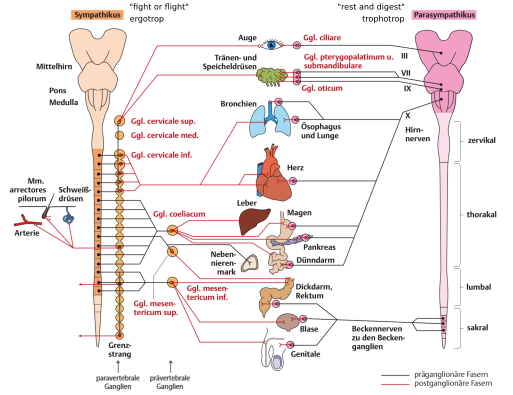
\includegraphics[width=0.8\textwidth]{Sympa_parasympa.png}
\end{center}

    
\end{frame}



%% SLide 2:

%% Übersicht to end all Übersichten: Emanuel Lecture 2 slide 6
%% Neurotransmitter und Rezeptoren
%% Peripheres NS: Verschaltung über Gaglion: Emanuel Slide 30
%% MUskarinerge Rezeptoren, Emanuel slide 35, anotate 
%% Adrenerge Rezepotiren, Emanuel slide 38
%% Cotransmitter: ATP; NO, Neuropeptide
%% Pharmacology: Indirekte, direkte Pharmakomimetika, Pharamtolytika


\begin{frame}{M11.11 Vegetatives Nervensystem 1: Peripheres Nervensystem}

\begin{center}
    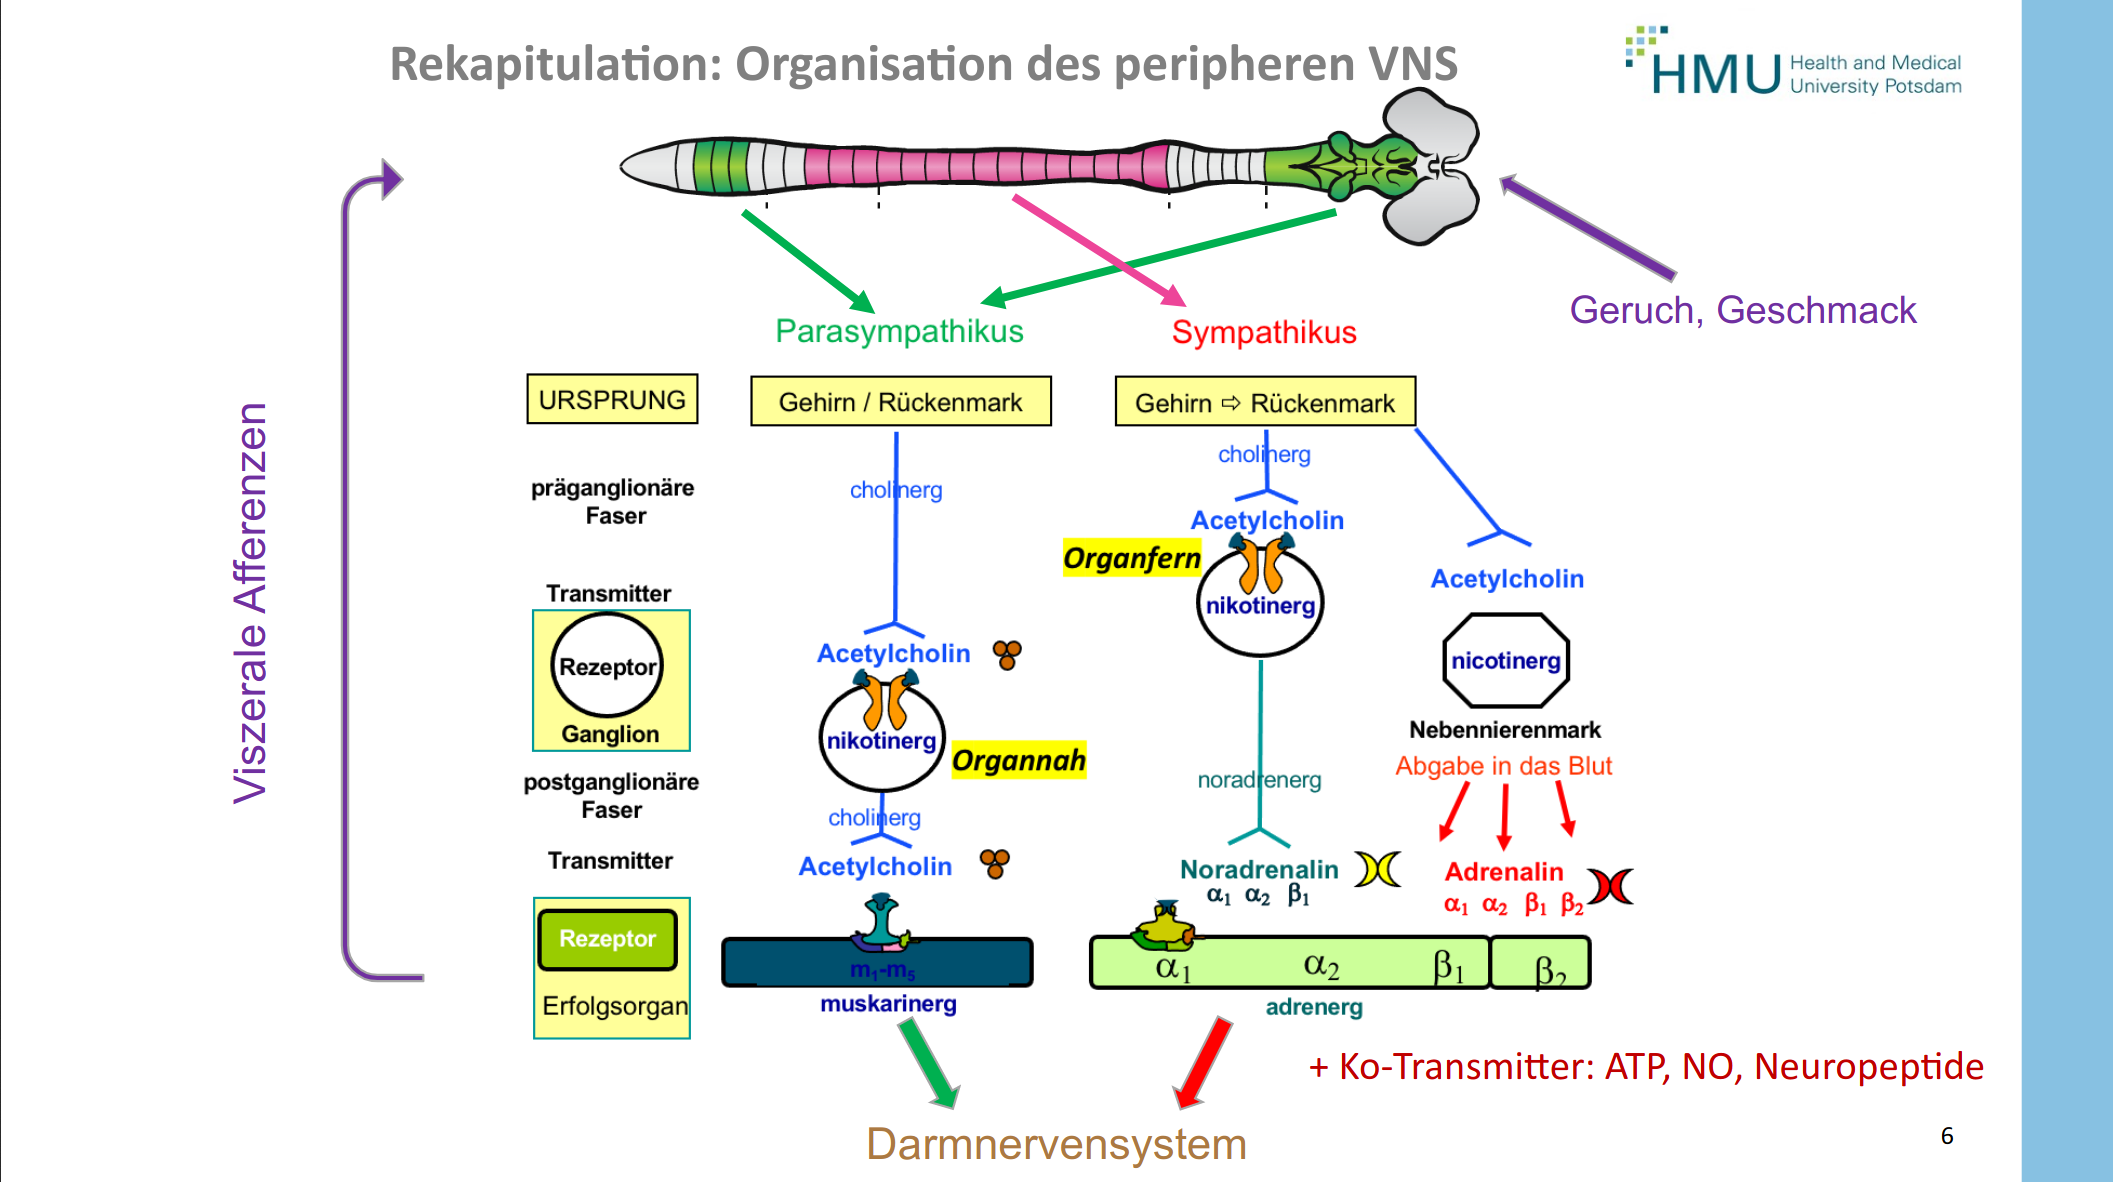
\includegraphics[width=\textwidth]{peripheres_VNS.png}
\end{center}

    
\end{frame}



%% IMPP: 



%% Verschaltung Sympathikus Parasympathikus: 286

\begin{frame}{IMPP Fragen}
\textbf{Die synaptische Übertragung von prä- auf postganglionäre Neurone es vegetativen Nervensystems erfolgt beim Menschen meistens} \\[0.2 cm]

\begin{itemize}
\item[A.] im Parasympathikus über muscarinische Acetylcholinrezeptoren
\item[B.] im Sympathikus über \(\alpha\)-Adrenozeptoren
\item[C.] im Sympathikus über \(\beta\)-Adrenozeptoren
\item[D.] im Sympathikus über muscarinische Acetylcholinrezeptoren
\item[E.] im Sympathikus über nicotinische Acetylcholinrezeptoren %% correct

\end{itemize}
\end{frame}

\begin{frame}{IMPP Fragen}
\textbf{Die synaptische Übertragung von prä- auf postganglionäre Neurone es vegetativen Nervensystems erfolgt beim Menschen meistens} \\[0.2 cm]

\begin{itemize}
\item[A.] im Parasympathikus über muscarinische Acetylcholinrezeptoren
\item[B.] im Sympathikus über \(\alpha\)-Adrenorezeptoren
\item[C.] im Sympathikus über \(\beta\)-Adrenorezeptoren
\item[D.] im Sympathikus über muscarinische Acetylcholinrezeptoren
\item[E.] \textcolor{blue}{im Sympathikus über nicotinische Acetylcholinrezeptoren} \\ %% correct
\pause
\textcolor{blue}{Und im Parasympathikus übrigens auch!}
\end{itemize}
\end{frame}


%% Sympathikus Neurotransmiter: new 26

\begin{frame}{IMPP Fragen}
\textbf{Welche Aussage über Adrenozeptoren trifft typischerweise zu?} \\[0.2 cm]

\begin{itemize}
\item[A.] Die Aktivierung von präsynaptischen \(\alpha_2\)-Adrenozeptoren auf sympathischen postganglionären Varikositäten fördert die Freisetzung von Noradrenalin. 
\item[B.] Die Aktivierung von präsynaptischen \(\beta\)-Adrenozeptoren auf sympathischen  postganglionären Varikositäten hemmt die Freisetzung von Noradrenalin. 
\item[C.] Die Aktivierung von \(\alpha_1\)-Adrenozeptoren auf glatten Muskelzellen hemmt die Bildung von Inositol-1,4,5-trisphosphat.
\item[D.] Die Aktivierung von \(\beta\)-Adrenozeptoren auf glatten Muskelzellen führt zur Aktivierung stimulierender G-Proteine (G\textsubscript{S}-Proteine).
\item[E.] Die synaptische Übertragung der sympathischen postganglionären Neurone auf die postganglionären Neurone wird durch Adrenozeptoren vermittelt. 

\end{itemize}
\end{frame}


\begin{frame}{IMPP Fragen}
\textbf{Welche Aussage über Adrenozeptoren trifft typischerweise zu?} \\[0.2 cm]

\begin{itemize}
\item[A.] Die Aktivierung von präsynaptischen \(\alpha_2\)-Adrenozeptoren auf sympathischen postganglionären Varikositäten fördert die Freisetzung von Noradrenalin. 
\item[B.] Die Aktivierung von präsynaptischen \(\beta\)-Adrenozeptoren auf sympathischen  postganglionären Varikositäten hemmt die Freisetzung von Noradrenalin. 
\item[C.] Die Aktivierung von \(\alpha_1\)-Adrenozeptoren auf glatten Muskelzellen hemmt die Bildung von Inositol-1,4,5-trisphosphat.
\item[D.] \textcolor{blue}{Die Aktivierung von \(\beta\)-Adrenozeptoren auf glatten Muskelzellen führt zur Aktivierung stimulierender G-Proteine (G\textsubscript{S}-Proteine).}
\item[E.] Die synaptische Übertragung der sympathischen postganglionären Neurone auf die postganglionären Neurone wird durch Adrenozeptoren vermittelt. 

\end{itemize}
\end{frame}




%%%%%%%%%%%%%%%%%%%%%%%%%%%%%%%%%%%%%%%%%%%%%%%%%%
%%%%%%%%%%%%%%%%%%%%%%%%%%%%%%%%%%%%%%%%%%%%%%%%%%
%%%%%%%%%%%%%%%%%%%%%%%%%%%%%%%%%%%%%%%%%%%%%%%%%%

%% Vegetatives Nervensystem 2: Vegetative Zentren und Organregulation


%% Lernziele: 

% Welches sind die zentralen Komponenten des vegetaAven Nervensystems
% und wie steuern sie dessen FunkAon?
% •
% Limbisches System
% •
% •
% Hirnstamm
% •
% •
% Hypothalamus
% Medulla oblongata
% Rückenmark
% Wie steuert das VNS OrganfunkAonen?
% • Herz-Kreislauf-System
% • Magen-Darm-Trakt
% Wie verändern sich vegetaAve Reflexbahnen bei Querschnittlähmung?

 
%% Slide 1 
%% Hierarchischer Aufbau des VNS - Slide 9
%% Lage und Anatomie des limbischen Systems . slide 14 mit Hypothalamus
%% Unterteilung des Hypothalamus? (S. 18)
\begin{frame}{M11.11 Vegetatives Nervensystem 2 Vegetative Zentren und Organregulation}
    \begin{columns}[c]
    
    \begin{column}{5cm}
    \begin{center}
        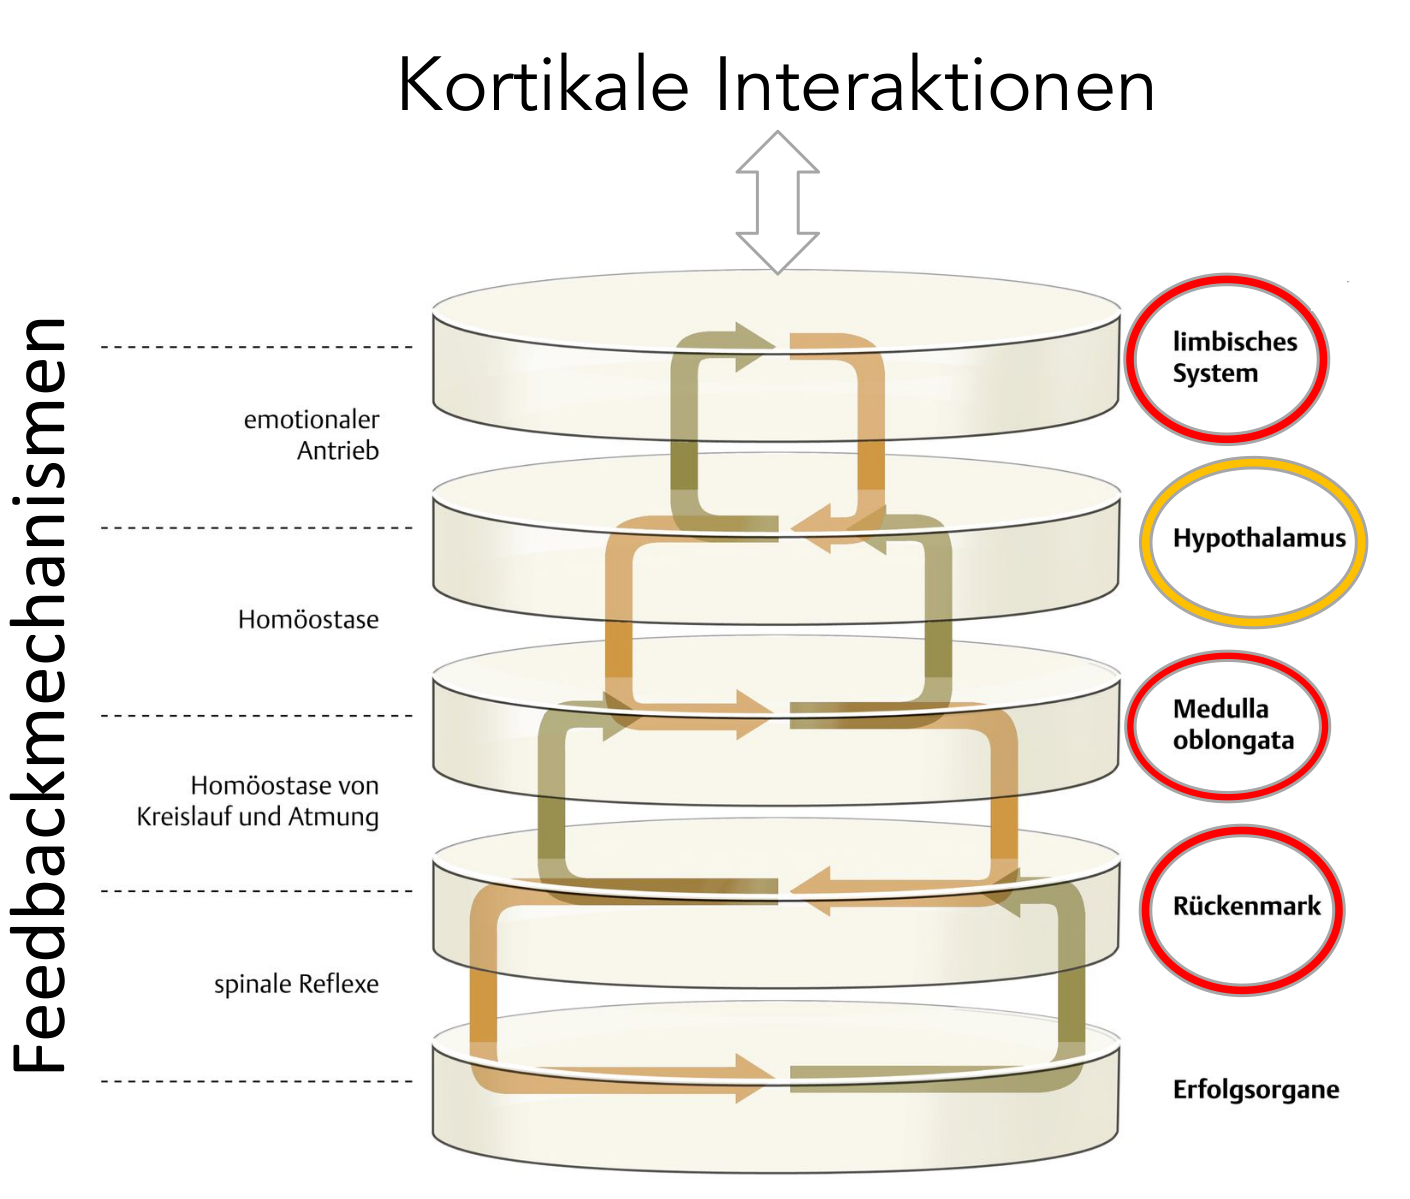
\includegraphics[width=\textwidth]{vns2_zentren.png}
    \end{center}
    \end{column}
    
    \begin{column}{5cm}
    
    \begin{center}
        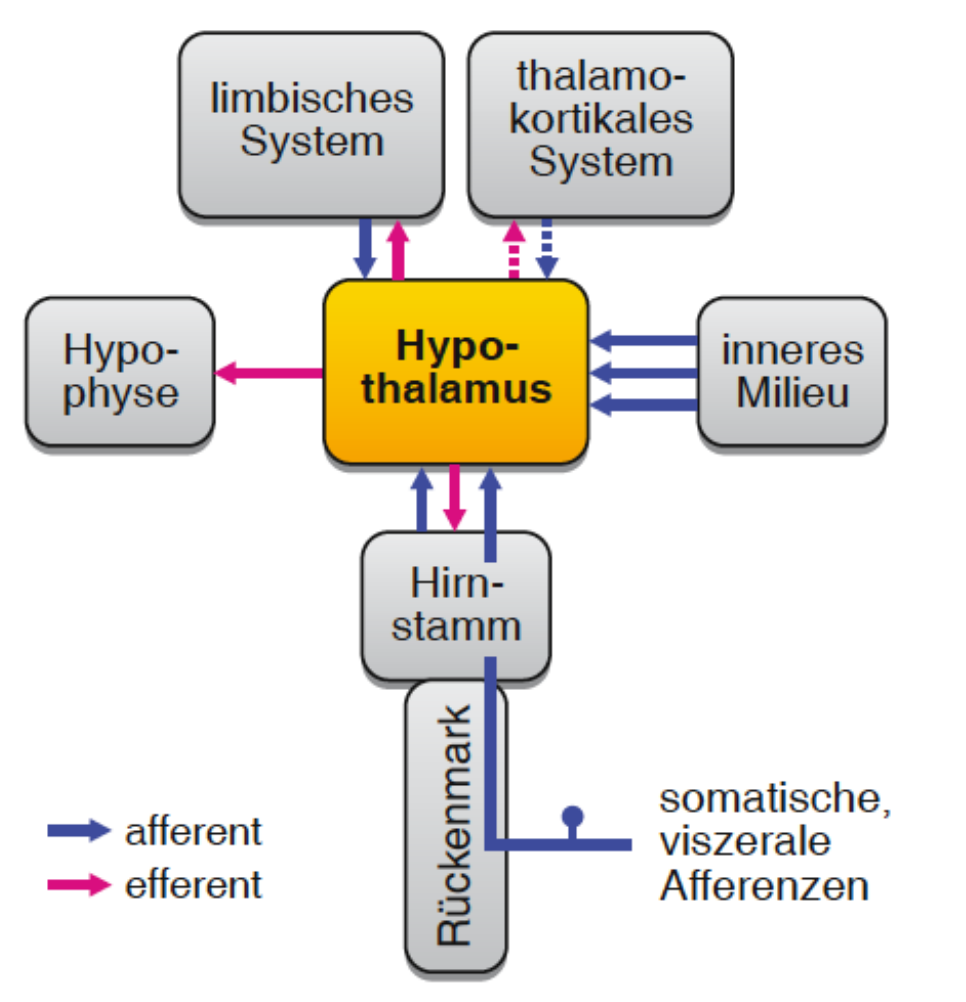
\includegraphics[width=\textwidth]{hypothalamus_nabel_der_welt.png}
    \end{center}
    
    
    
    \end{column}
    
    
    \end{columns}
    
    
    
\end{frame}



% %% Slide 2: Herz- Kreislaufsystem, Defäkation, miktion
% \begin{frame}{M11.11 Vegetatives Nervensystem 2 Vegetative Zentren und Organregulation}

% \begin{columns}[c]
% \begin{column}{5cm}
% %% Zielorgane allgemein
%     \begin{center}
%         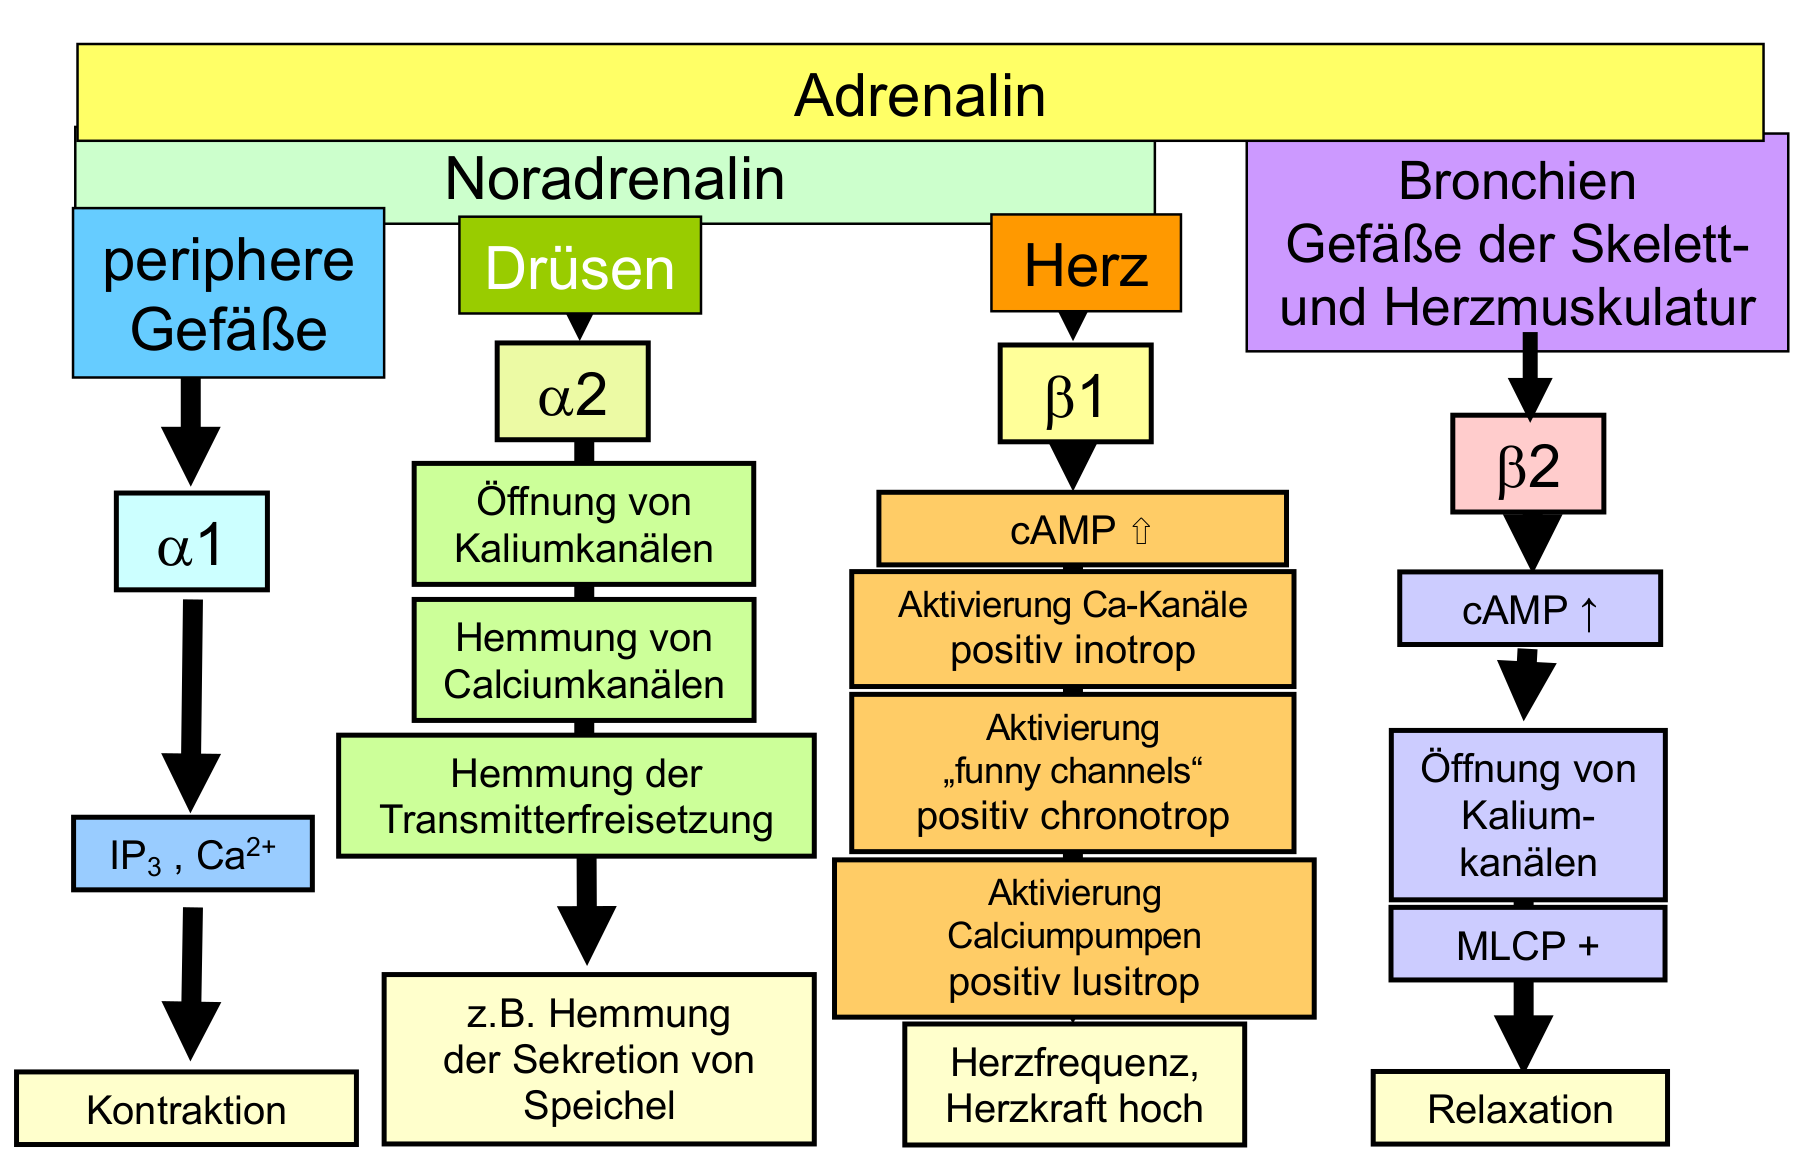
\includegraphics[width=\textwidth]{adrenerge_systeme.png}
%     \end{center}
    
%         \begin{center}
%         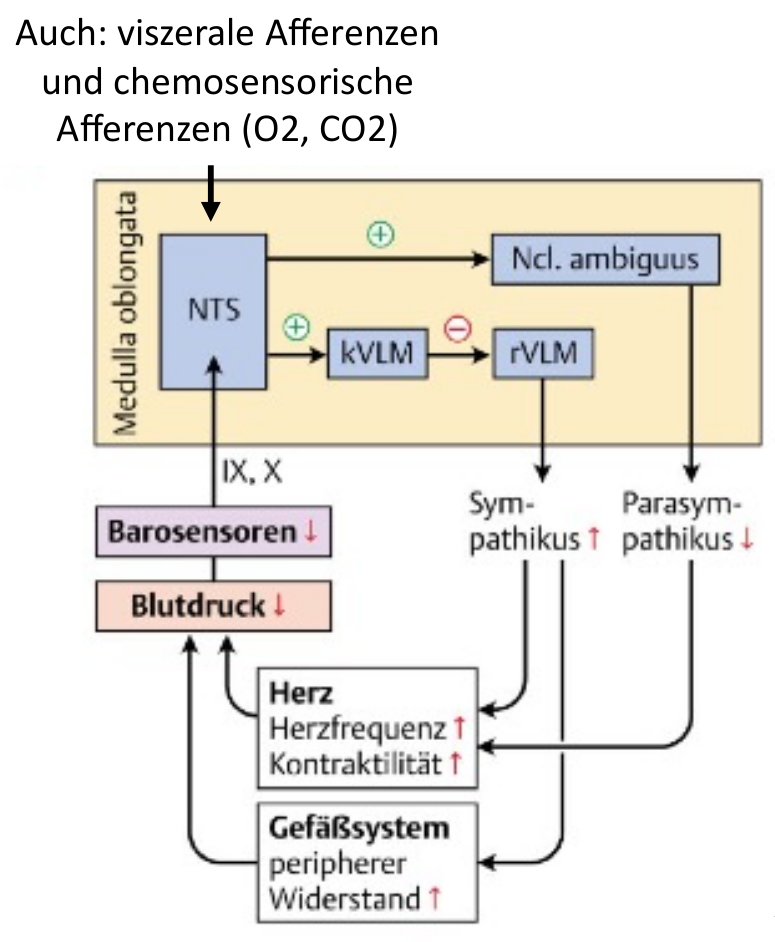
\includegraphics[width=\textwidth]{kreislauf.png}
%     \end{center}
% %% Herz-Kreislauf
% \end{column}

% \begin{column}{5cm}
% %% Defäkation



% %% Miktion
% \end{column}



% \end{columns}




% \end{frame}


%% New 20: Pressorezeptoren
\begin{frame}{IMPP Fragen}


\textbf{Welche Aussage über arterielle Pressorezeptoren (Barosensoren) trifft typischerweise zu?} \\[0.2 cm]

\begin{itemize}
\item[A.] Ihre Aktivierung steigert die Aktivität der postganglionären efferenten sympathischen Fasern zum Herzen.
\item[B.] Sie besitzen mechanosensitive Kationenkanäle. %% correct
\item[C.] Sie reagieren auf Erhöhung des statischen Drucks mit einer Abnahme der Entladungsfrequenz ihrer Afferenzen.
\item[D.] Sie zeigen bei konstanter Reizstärke keine Adaptation.
\item[E.] Sie zeigen kein Differentialverhalten.

\end{itemize}


\end{frame}


\begin{frame}{IMPP Fragen}


\textbf{Welche Aussage über arterielle Pressorezeptoren (Barosensoren) trifft typischerweise zu?} \\[0.2 cm]

\begin{itemize}
\item[A.] Ihre Aktivierung steigert die Aktivität der postganglionären efferenten sympathischen Fasern zum Herzen.
\item[B.] \textcolor{blue}{Sie besitzen mechanosensitive Kationenkanäle.} %% correct
\item[C.] Sie reagieren auf Erhöhung des statischen Drucks mit einer Abnahme der Entladungsfrequenz ihrer Afferenzen.
\item[D.] Sie zeigen bei konstanter Reizstärke keine Adaptation.
\item[E.] Sie zeigen kein Differentialverhalten.

\end{itemize}


\end{frame}


%% Details: Rezeptoren New 30


\begin{frame}{IMPP Fragen}


\textbf{Bei den adrenergen Rezeptoren werden mehrere Isoformen unterschieden (u.a. \(\alpha_1\)-, \(\alpha_2\)-, \(\beta_1\)-, \(\beta_2\)- und \(\beta_3\)-Rezeptoren). }

\textbf{An welchen der folgenden Zellen wird die jeweils genannte, durch Stimulation ihrer adrenergen Rezeptoren hervorgerufene Wirkung typischerweise über \(\alpha_1\)-Rezeptoren vermittelt?} \\[0.2 cm]

\begin{itemize}
\item[A.] Bronchialmuskelzellen \(\rightarrow\) Bronchodilatation
\item[B.] glatte Gefäßmuskelzellen der Nierenarterien \(\rightarrow\) Vasokonstriktion %% correct 
\item[C.]  glatte Gefäßmuskelzellen  im Skelettmuskel \(\rightarrow\) Vasodilatation
\item[D.]  kardiale Sinusknotenzellen \(\rightarrow\) Beschleunigung der Herzfrequenz
\item[E.] Uterusmuskelzellen \(\rightarrow\) Erschlaffung der Uterusmuskulatur 

\end{itemize}


\end{frame}


\begin{frame}{IMPP Fragen}


\textbf{Bei den adrenergen Rezeptoren werden mehrere Isoformen unterschieden (u.a. \(\alpha_1\)-, \(\alpha_2\)-, \(\beta_1\)-, \(\beta_2\)- und \(\beta_3\)-Rezeptoren). }

\textbf{An welchen der folgenden Zellen wird die jeweils genannte, durch Stimulation ihrer adrenergen Rezeptoren hervorgerufene Wirkung typischerweise über \(\alpha_1\)-Rezeptoren vermittelt?} \\[0.2 cm]

\begin{itemize}
\item[A.] Bronchialmuskelzellen \(\rightarrow\) Bronchodilatation
\item[B.] \textcolor{blue}{glatte Gefäßmuskelzellen der Nierenarterien \(\rightarrow\) Vasokonstriktion} %% correct 
\item[C.]  glatte Gefäßmuskelzellen  im Skelettmuskel \(\rightarrow\) Vasodilatation
\item[D.]  kardiale Sinusknotenzellen \(\rightarrow\) Beschleunigung der Herzfrequenz
\item[E.] Uterusmuskelzellen \(\rightarrow\) Erschlaffung der Uterusmuskulatur 

\end{itemize}


\end{frame}






%%%%%%%%%%%%%%%%%%%%%%%%%%%%%%%%%%%%%%%%%%%%%%%%%%
%%%%%%%%%%%%%%%%%%%%%%%%%%%%%%%%%%%%%%%%%%%%%%%%%%
%%%%%%%%%%%%%%%%%%%%%%%%%%%%%%%%%%%%%%%%%%%%%%%%%%


%% Schlaf und EEG
\section{}

%% EEG 
%% Ableitung
%% Synchrone, asynchrone Aktivität

\begin{frame}{M11.11 ZNS 2: Schlaf und EEG} 

\begin{columns}[c]

\begin{column}{5cm}

\begin{center}
    
    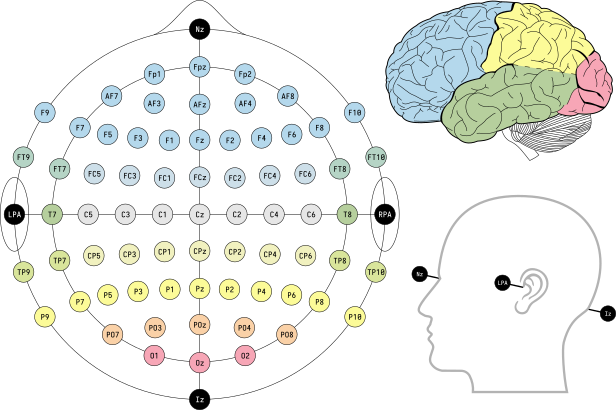
\includegraphics[width=\textwidth]{EEG_10-10_system.png}
    
    
    \end{center}
    
    $\,$\\
    
    \begin{center}
        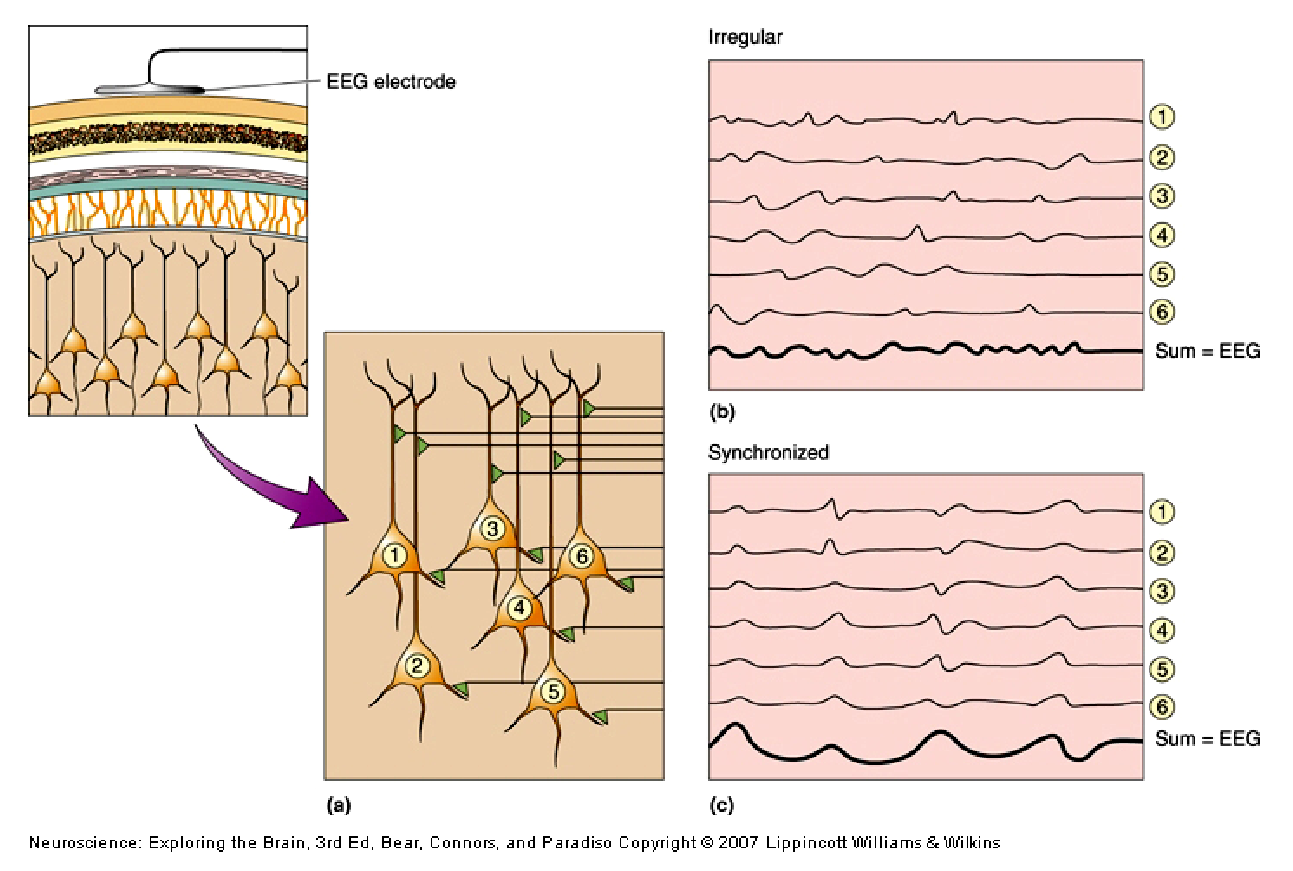
\includegraphics[width=\textwidth]{EEG_synchrony..png}

\end{center}

\end{column}

\begin{column}{6cm}

EEG misst Summe aus vielen synchronen EPSPs.   \\
Amplitude: \\ \(50-100\,\mu V\) (Hintergrund-EEG), \\ \(1-15\mu V\) (evozierte Potentiale) \\
Räumliche Auflösung: cm-Bereich \\
Zeitliche Auflösung: \(0.5-30\,\)Hz \\ \pause
Bei neurologische Krankheiten oft atypisches EEG, z.B. Epilepsie 


\begin{center}
    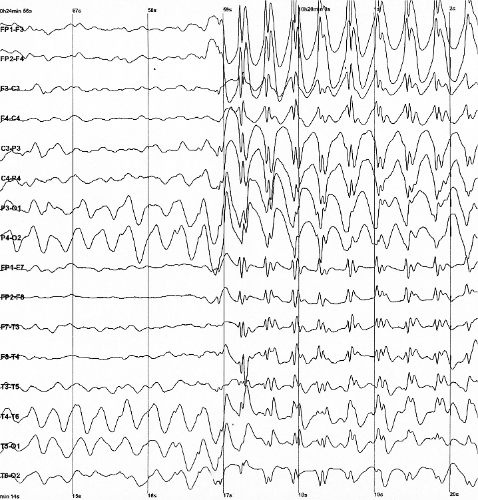
\includegraphics[width=0.6\textwidth]{Spike-waves.png}
\end{center}


\end{column}


\end{columns}

\end{frame}




%% Schlaf und Epilepsie
%% ARAS; Übergang zwischen Schlafphasen, EEG bei Schlaf 
\begin{frame}{M11.11 ZNS 2: Schlaf und EEG}
    
    %% both formatio reticularis slides
    \begin{columns}[c]
    \begin{column}{6cm}
    
    \begin{center}
        \includegraphics<1>[width=\textwidth]{formatio_reticularis_1.pdf}
        \includegraphics<2->[width=\textwidth]{formatio_reticularis_2.pdf}
    \end{center}
    
    \pause
    
    
    \end{column}
    
    \begin{column}{5cm}
    
    \pause
    
    \begin{block}{Schlaf EEG}
    
    \begin{center}
        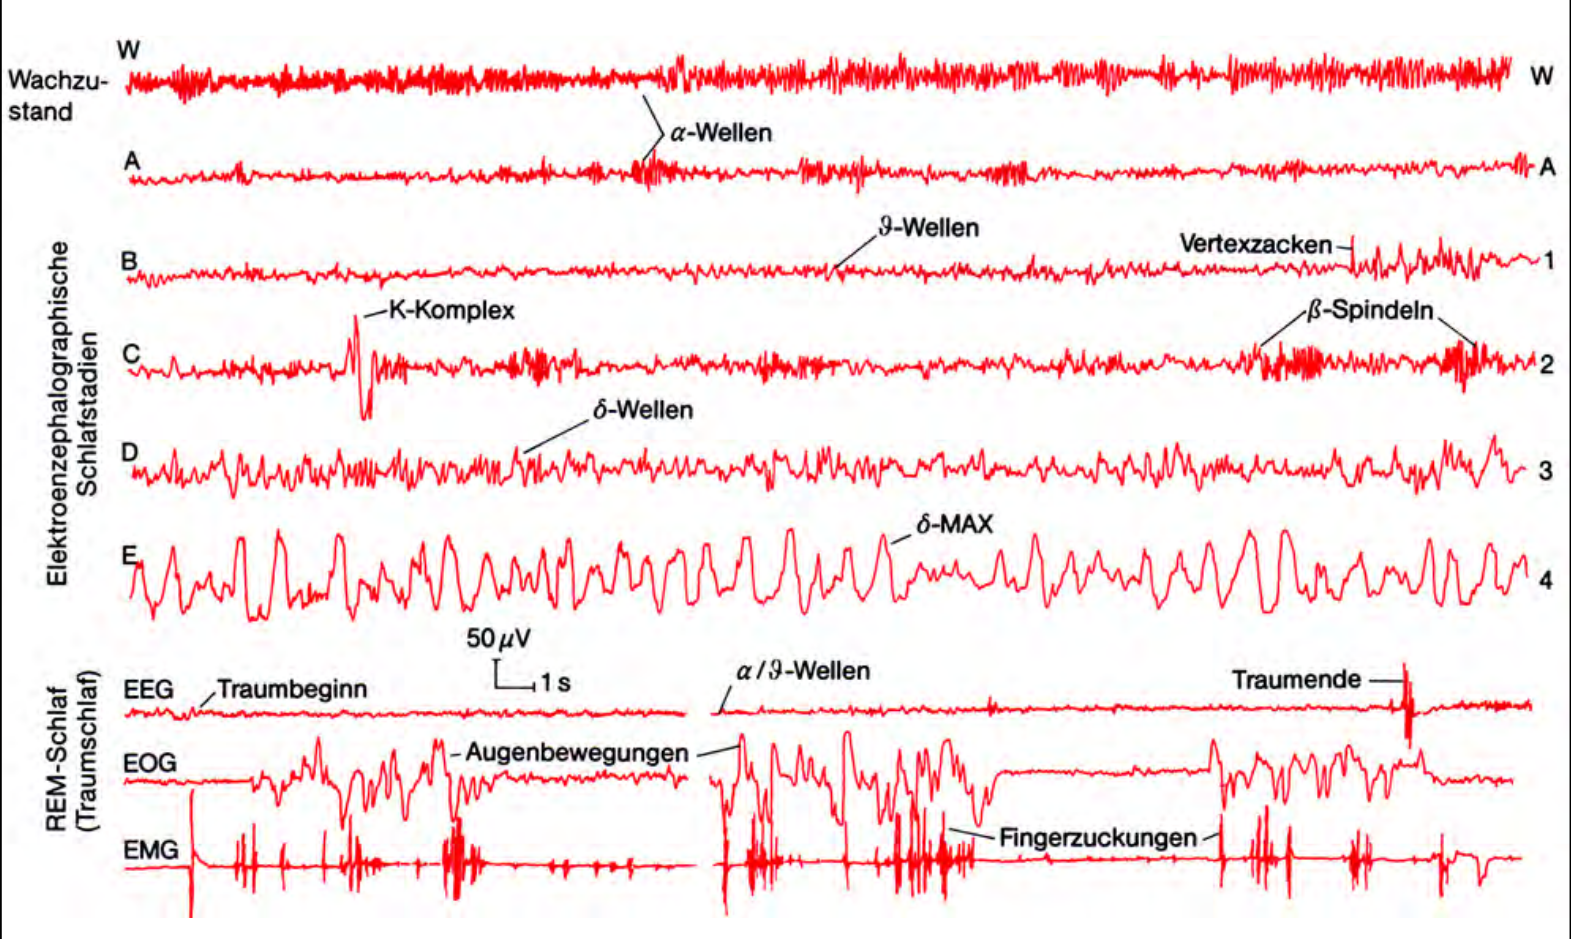
\includegraphics[width=\textwidth]{schlaf_eeg.png}
    \end{center}
    
    \end{block}
    
    \end{column}
    
    
    \end{columns}
    
    
    \pause

\begin{block}{Kontrolle der Schlafphasen}
\begin{columns}[c]
\begin{column}{3cm}
    \begin{center}
        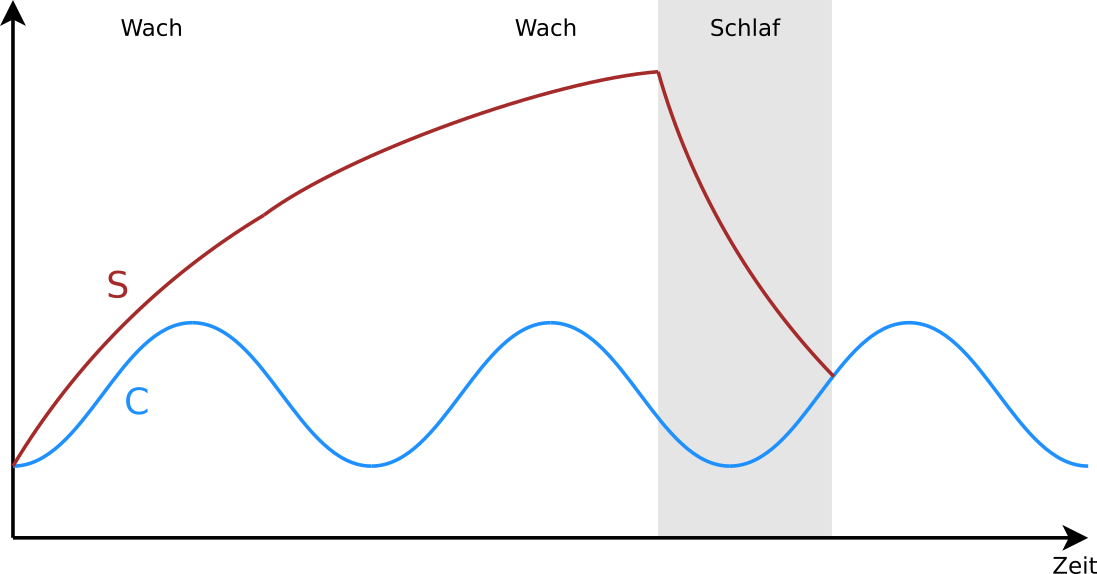
\includegraphics[width=\textwidth]{Zwei-prozess-2.png}
    \end{center}
    
    \end{column}
    
    \begin{column}{8cm}
    Homöostatischer Faktor: Adenosin  \\
    Rhythmischer Faktor: Circadianer Rhythmus \\
    Übergang zwischen REM und non-REM Schlaf wird im Pons kontrolliert. 


    
    \end{column}
    
    \end{columns}
    



    
    
    \end{block}
    
\end{frame}



%% EEG allgemein - 112
\begin{frame}{IMPP Fragen}

\textbf{
Welche Aussage zum (in üblicher Weise abgeleiteten) EEG eines Gesunden trifft am ehesten zu?
} \\[0.2 cm]

\begin{itemize}
\item[A.] Die räumliche Auflösung des EEG ermöglicht die Lokalisation einzelner kortikaler Neurone
\item[B.] Im Wachzustand haben die Potenzialschwankungen im EEG eine durchschnittliche Amplitude von \(5-10\,mV\)
\item[C.] \(\beta\)-Wellen haben durchschnittlich höhere Amplituden als \(\alpha\)-Wellen
\item[D.] Wellen mit einer Amplitude von über \(100\,\mu V\) lassen sich im EEG nur bei wachen Personen ableiten
\item[E.] Zum Auftreten von \(\alpha\)-Wellen im EEG trägt die synchrone Aktivität thalamokortikaler Verbindungen bei. %% correct

\end{itemize}

\end{frame}


\begin{frame}{IMPP Fragen}

\textbf{
Welche Aussage zum (in üblicher Weise abgeleiteten) EEG eines Gesunden trifft am ehesten zu?
} \\[0.2 cm]

\begin{itemize}
\item[A.] Die räumliche Auflösung des EEG ermöglicht die Lokalisation einzelner kortikaler Neurone
\item[B.] Im Wachzustand haben die Potenzialschwankungen im EEG eine durchschnittliche Amplitude von \(5-10\,mV\)
\item[C.] \(\beta\)-Wellen haben durchschnittlich höhere Amplituden als \(\alpha\)-Wellen
\item[D.] Wellen mit einer Amplitude von über \(100\,\mu V\) lassen sich im EEG nur bei wachen Personen ableiten
\item[E.] \textcolor{blue}{Zum Auftreten von \(\alpha\)-Wellen im EEG trägt die synchrone Aktivität thalamokortikaler Verbindungen bei.} %% correct

\end{itemize}

\end{frame}



%% Schlaf

\begin{frame}{IMPP Fragen}

\textbf{Sie sitzen vor dem Computer im Schlaflabor und analysieren ein EEG eines Patienten. Dabei beobachten Sie überwiegend Wellen im Frequenzbereich zwischen 8 und 12\,Hz. }
\textbf{Welcher Bewusstseinsgrad ist für den Patienten am ehesten zutreffend?} \\[0.2 cm]

\begin{itemize}
\item[A.] Aktivation
\item[B.] entspannter Wachzustand
\item[C.] Ermüdung
\item[D.] hohe Aufmerksamkeit
\item[E.] Tiefschlaf
\end{itemize}

\end{frame}


\begin{frame}{IMPP Fragen}

\textbf{Sie sitzen vor dem Computer im Schlaflabor und analysieren ein EEG eines Patienten. Dabei beobachten Sie überwiegend Wellen im Frequenzbereich zwischen 8 und 12\,Hz. }
\textbf{Welcher Bewusstseinsgrad ist für den Patienten am ehesten zutreffend?} \\[0.2 cm]

\begin{itemize}
\item[A.] Aktivation
\item[B.] \textcolor{blue}{entspannter Wachzustand  - \(\alpha\)-Wellen}  
\item[C.] Ermüdung
\item[D.] hohe Aufmerksamkeit
\item[E.] Tiefschlaf
\end{itemize}

\end{frame}



%%%%%%%%%%%%%%%%%%%%%%%%%%%%%%%%%%%%%%%%%%%%%%%%%%
%%%%%%%%%%%%%%%%%%%%%%%%%%%%%%%%%%%%%%%%%%%%%%%%%%
%%%%%%%%%%%%%%%%%%%%%%%%%%%%%%%%%%%%%%%%%%%%%%%%%%


%% Lernen und Plastizität

%% Slide 1
%%  Arten von Gedächtnis, Arten des Lernens: Zeit (+ Aufmerksamkeit), assoziativ, nicht-assoziativ, Modelllernen
\begin{frame}{M11.11 ZNS 3: Lernen und Plastizität} 

\begin{columns}[c]

\begin{column}{5cm}
\begin{center}
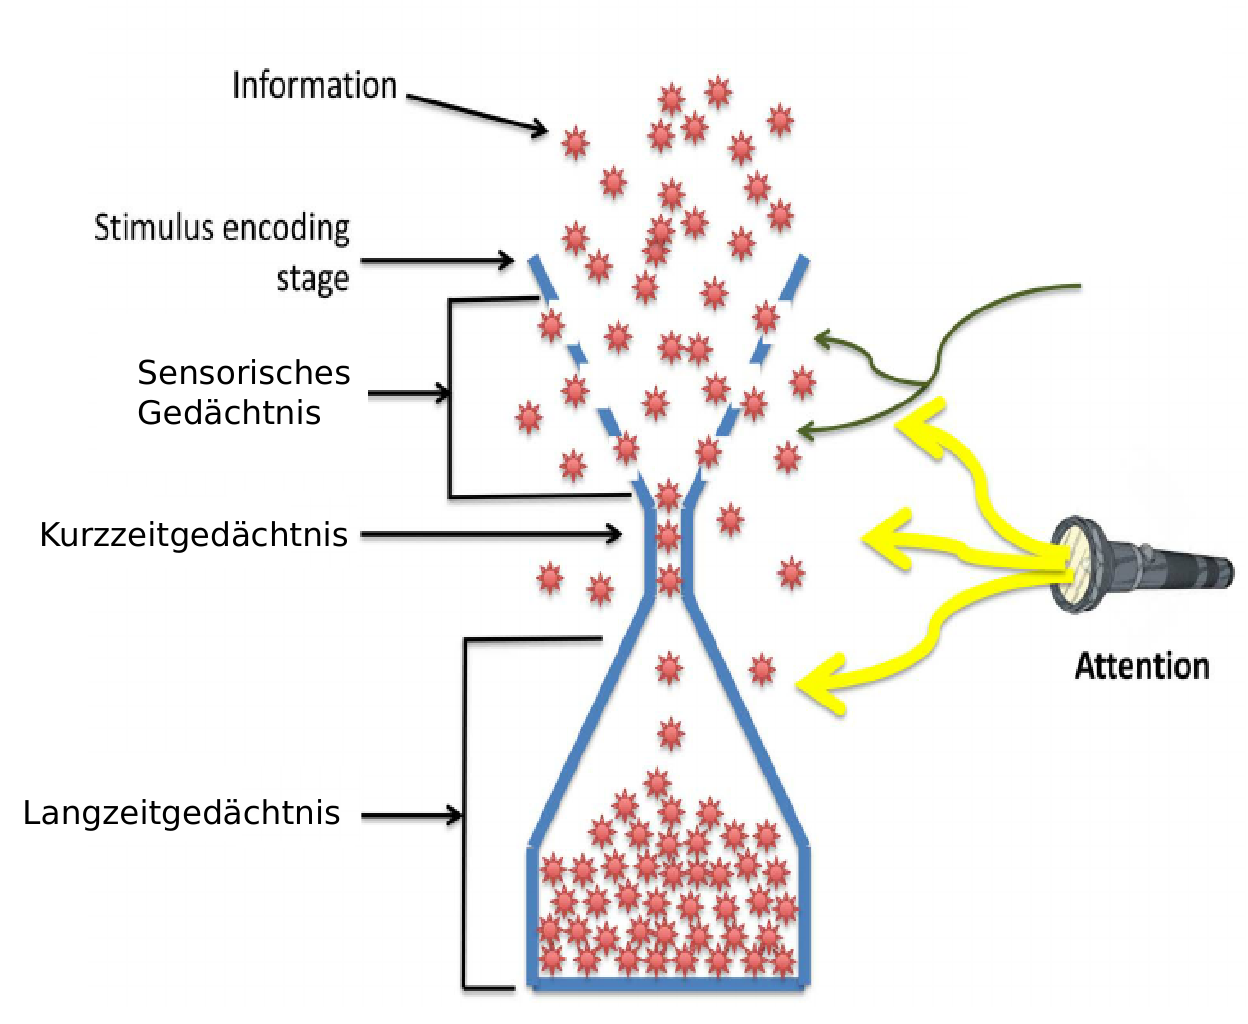
\includegraphics[width=\textwidth]{ultrakurzlang.png}
\end{center}

\begin{center}
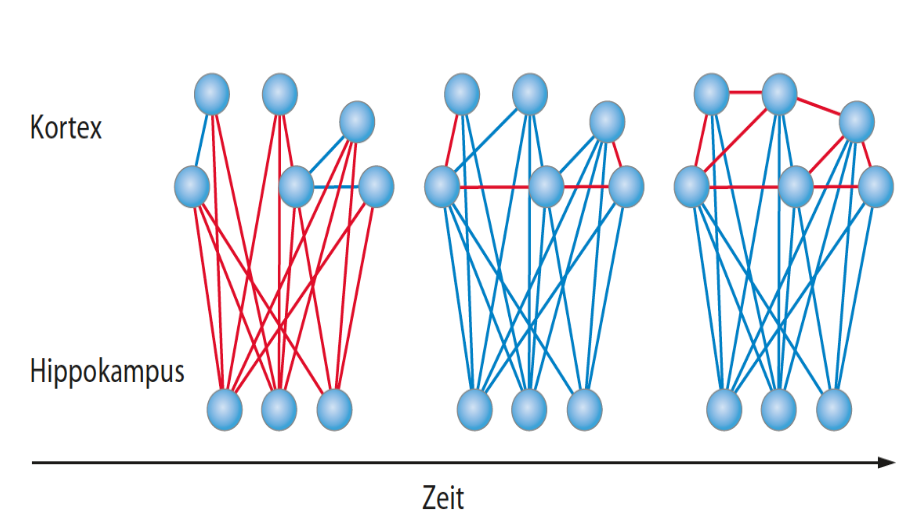
\includegraphics[width=\textwidth]{konsolidierung.png}
\end{center}


\end{column}

\begin{column}{5cm}
\begin{block}{Explizites (delkaratives) Gedächtnis}
Semantisch (Fakten)
Episodisch (Erlebnisse)
\end{block}

\begin{block}{Implizites Gedächtnis}
Perzeptuell (Mustererkennung) \\
Prozedural (Fertigkeiten) \\
Priming (Wiedererkennung) \\
Assoziativ (Emotionale Reflexe) \\
Habituation (Gewöhnung)
\end{block}



\end{column}


\end{columns}


\end{frame}



%% Slide 2

%% Hebbsche Synapse, LTP + Molekular
\begin{frame}{M11.11 ZNS 3: Lernen und Plastizität} 

\begin{center}
    \includegraphics<1>[width=\textwidth]{LTP1_AMPAR.png}
    \includegraphics<2>[width=\textwidth]{LTP2_depol.png}
    \includegraphics<3>[width=\textwidth]{LTP3_NMDAR.png}
    \includegraphics<4>[width=\textwidth]{LTP4_Ca.png}
    \includegraphics<5>[width=\textwidth]{LTP5_Calm.png}
    \includegraphics<6>[width=\textwidth]{signalling_general_SBGN_compliant.png}
\end{center}

\end{frame}


%% IMPP Fragen

%% Allgemein: Implizites Lernen: 358
\begin{frame}{IMPP Fragen}

\textbf{Welche der Aussagen über das implizite Lernen bzw. Gedächtnis trifft am ehesten zu?} \\[0.2 cm]

\begin{itemize}
\item[A.] Bei beidseitiger Schädigung de Hippocampus ist implizites Lernen nicht mehr möglich.
\item[B.] Bei Patienten mit anterograder Amnesie ist implizites Lernen nicht mehr möglich.
\item[C.] Beim impliziten Lernen ist vor allem die mediale Temporallappenregion aktiv.
\item[D.] Das prozedurale Gedächtnis speichert typischerweise Fakten.
\item[E.] Implizite Lernvorgänge beruhen u.a. auf Plastizität in Basalganglien und Zerebellum %% correct

\end{itemize}

\end{frame}


\begin{frame}{IMPP Fragen}

\textbf{Welche der Aussagen über das implizite Lernen bzw. Gedächtnis trifft am ehesten zu?} \\[0.2 cm]

\begin{itemize}
\item[A.] Bei beidseitiger Schädigung de Hippocampus ist implizites Lernen nicht mehr möglich.
\item[B.] Bei Patienten mit anterograder Amnesie ist implizites Lernen nicht mehr möglich.
\item[C.] Beim impliziten Lernen ist vor allem die mediale Temporallappenregion aktiv.
\item[D.] Das prozedurale Gedächtnis speichert typischerweise Fakten.
\item[E.] \textcolor{blue}{Implizite Lernvorgänge beruhen u.a. auf Plastizität in Basalganglien und Zerebellum} %% correct

\end{itemize}

\end{frame}



%% Mehr LTP 
%% 123

\begin{frame}{IMPP Fragen}

\textbf{Die Langzeitspeicherung von Informationen im menschlichen Gehirn erfolgt durch plastische Veränderungen an zentralen Synapsen.}

\textbf{Welcher der folgenden Prozesse ist typischerweise an der Auslösung der Langzeitpotenzierung (LTP) der synaptischen Übertragung in exzitatorischen Synapsen beteiligt? } \\[0.2 cm]

\begin{itemize}
\item[A.] Aufhebung des Mg\textsuperscript{2+}-Blocks der NMDA-Rezeptoren durch Aktivierung von AMPA-Rezeptoren
\item[B.] erniedrigte Ca\textsuperscript{2+}-Permeabilität von AMPA-Rezeptoren in der postsynaptischen Membran
\item[C.] Hyperpolarisation der postsynaptischen Membran durch retrograde Ausbreitung somatischer Aktionspotentiale
\item[D.] reduzierte Offenwahrscheinlichkeit präsynaptischer Calciumkanäle vom P/Q Typ
\item[E.] vermehrte Endozytose von AMPA-Rezeptoren an der postsynaptischen Membran

\end{itemize}

\end{frame}


\begin{frame}{IMPP Fragen}

\textbf{Die Langzeitspeicherung von Informationen im menschlichen Gehirn erfolgt durch plastische Veränderungen an zentralen Synapsen.}

\textbf{Welcher der folgenden Prozesse ist typischerweise an der Auslösung der Langzeitpotenzierung (LTP) der synaptischen Übertragung in exzitatorischen Synapsen beteiligt? } \\[0.2 cm]

\begin{itemize}
\item[A.] \textcolor{blue}{Aufhebung des Mg\textsuperscript{2+}-Blocks der NMDA-Rezeptoren durch Aktivierung von AMPA-Rezeptoren}
\item[B.] erniedrigte Ca\textsuperscript{2+}-Permeabilität von AMPA-Rezeptoren in der postsynaptischen Membran
\item[C.] Hyperpolarisation der postsynaptischen Membran durch retrograde Ausbreitung somatischer Aktionspotentiale
\item[D.] reduzierte Offenwahrscheinlichkeit präsynaptischer Calciumkanäle vom P/Q Typ
\item[E.] vermehrte Endozytose von AMPA-Rezeptoren an der postsynaptischen Membran

\end{itemize}

\end{frame}






%%%%%%%%%%%%%%%%%%%%%%%%%%%%%%%%%%%%%%%%%%%%%%%%%%
%%%%%%%%%%%%%%%%%%%%%%%%%%%%%%%%%%%%%%%%%%%%%%%%%%
%%%%%%%%%%%%%%%%%%%%%%%%%%%%%%%%%%%%%%%%%%%%%%%%%%


%% Motorik 1 

%% Sesnsorische Organe in Muskeln
%%  Vestibulärsystem, Cerebellum

\begin{frame}{M11.12 Motorik 1: Grundlagen und Reflexe} 


\begin{columns}[c]

\begin{column}{5cm}
\begin{block}{Muskelspindel}


Misst Dehnung (Ia, II) \\
% \(\gamma\)-Faser ermöglicht Sensitivität \\
Parallel zum Muskel \\

\begin{center}
    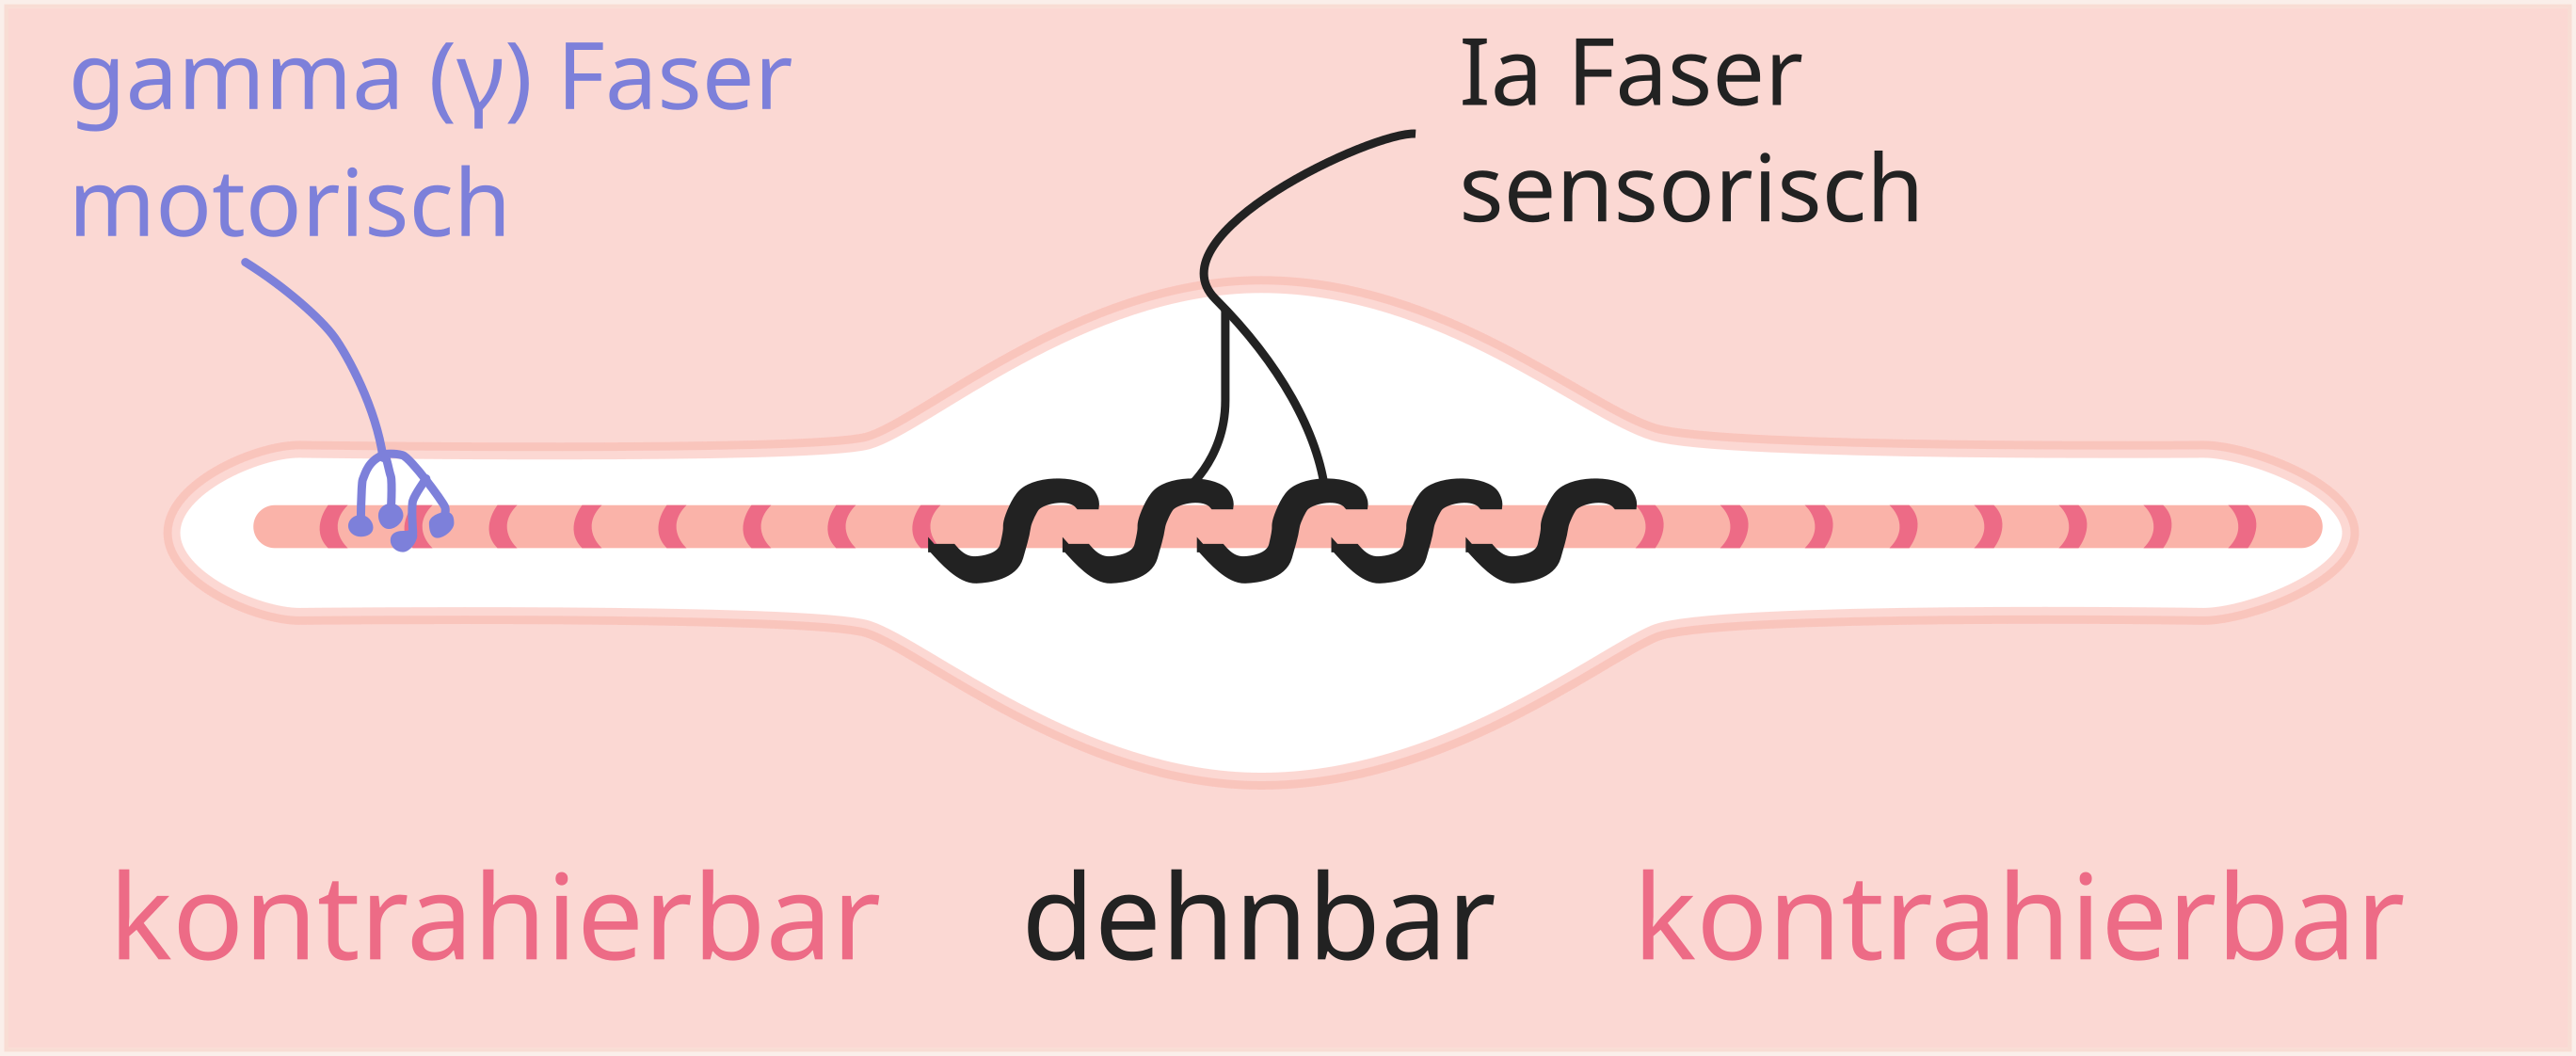
\includegraphics[width=\textwidth]{MuscleSpindle.png}
\end{center}

\end{block}

\begin{block}{Golgi-Sehnen-Organ}

Misst Spannung (Ib)\\
Seriell zum Muskel


\begin{center}
    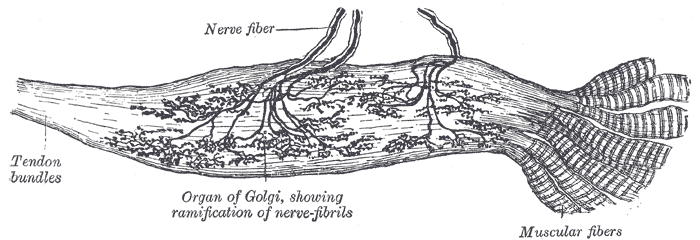
\includegraphics[width=0.8\textwidth]{Gray938.png}
\end{center}


\end{block}
\end{column}

\pause

\begin{column}{5cm}

\textbf{Vestibularsystem}: Gleichgewicht, Haltung  \\


\textbf{Cerebellum}: Kontrolle, Koordination, Feinabstimmung \\

\pause

\begin{center}
    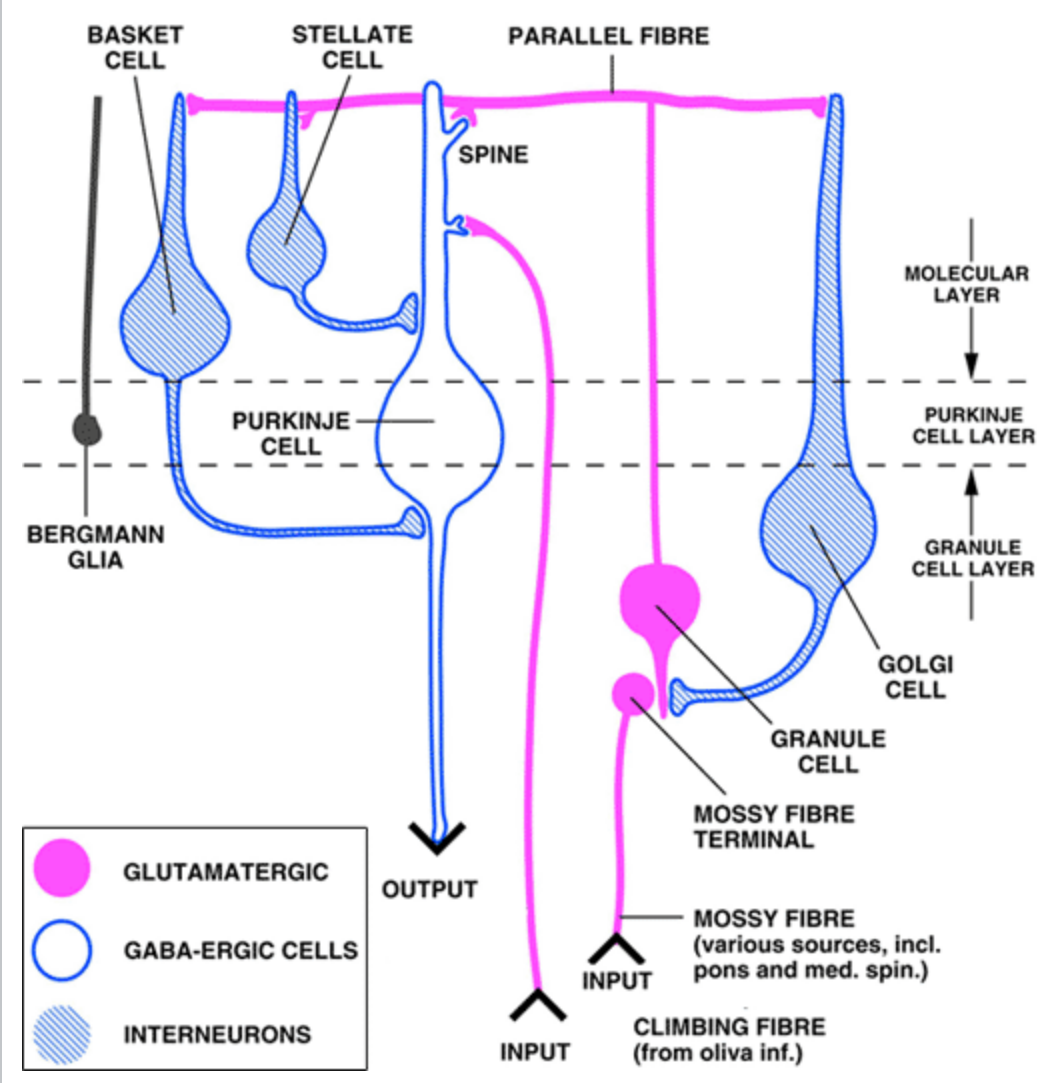
\includegraphics[width=\textwidth]{cerebellum_layers.png}
\end{center}

\end{column}


\end{columns}


\end{frame}



\begin{frame}{M11.12 Motorik 1: Grundlagen und Reflexe} 

%% Rückenmark
%%  Reflexbogen

\begin{columns}[t]
\begin{column}{5cm}
\textbf{Rückenmark} \\

\begin{center}
    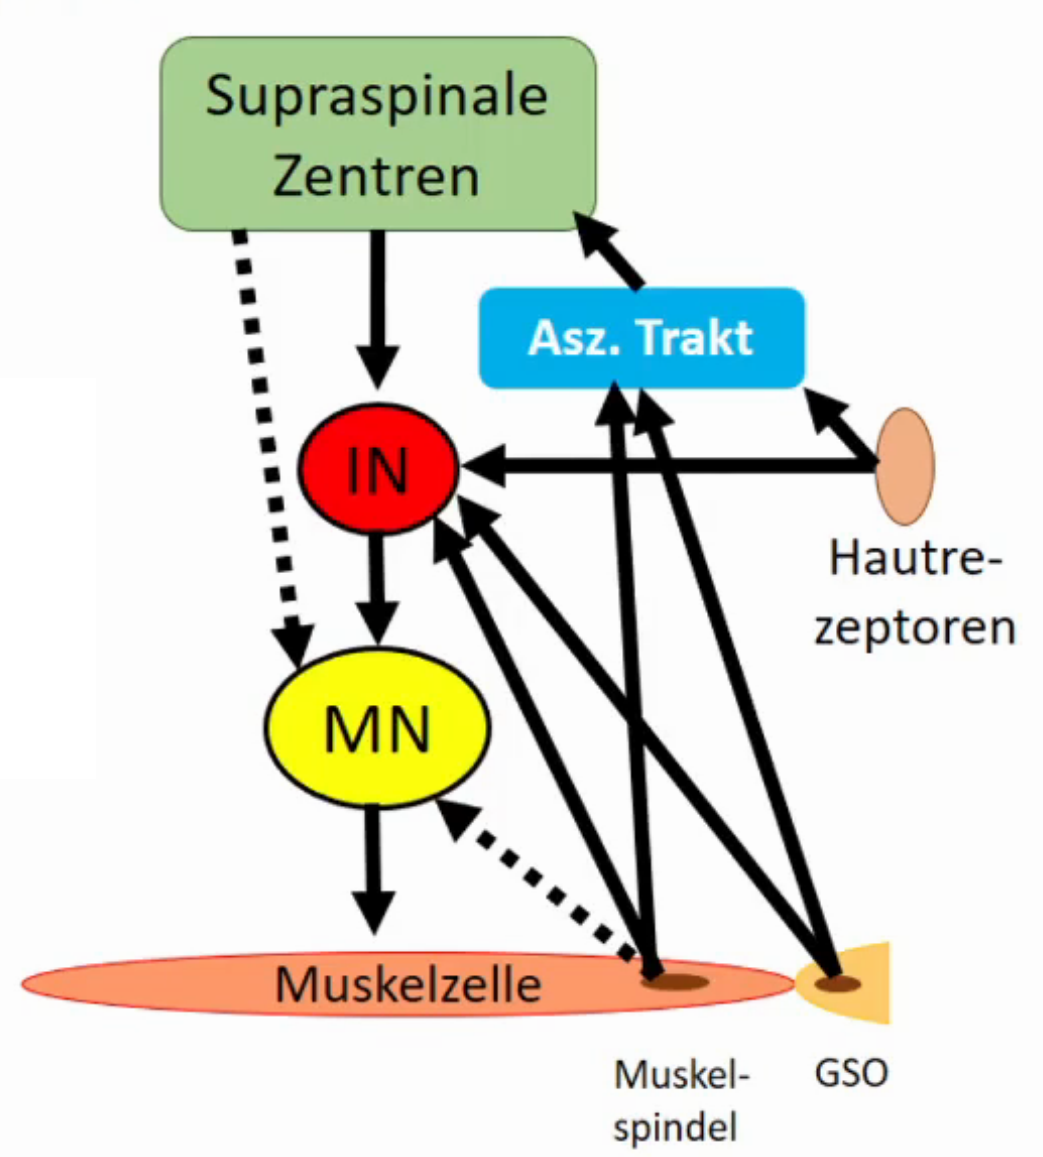
\includegraphics[width=\textwidth]{rueckenmark_orga.png}
\end{center}

\pause
\textbf{Supraspinale Reflexe}: Vestibulo-Okularer Reflex \\


\end{column}

\pause

\begin{column}{6cm}

\begin{center}
    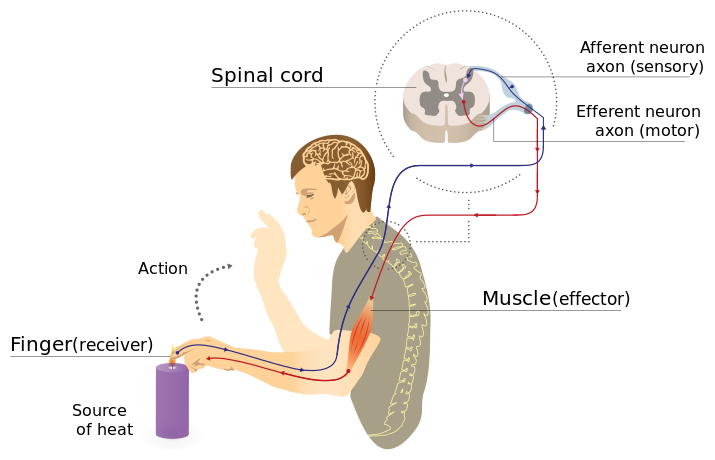
\includegraphics[width=\textwidth]{reflex_arc.png}
\end{center}

\textbf{Eigenreflexe}: Muskeldehnungsreflex, Rückwärtshemmung (Renshaw-Zellen), H-Reflex \\
\textbf{Fremdreflexe}: Beuge- und Streckreflex \\



\end{column}


\end{columns}
$\,$\\[0.2 cm]



%% Eigen-, Fremdreflexe




\end{frame}



%% 416 - Muskelspindeln
\begin{frame}{IMPP Fragen}

\textbf{Welche Aussage zu den Muskelspindeln trifft am ehesten zu?} \\[0.2 cm]

\begin{itemize}
\item[A.] Axone der Typ-II-Afferenzen innervieren vorwiegend die Kernsackfasern, jedoch kaum die Kernkettenfasern
\item[B.] Bei einer langsamen Präzisionsbewegung erfolgt (synchron zur Aktivierung der \(\alpha\)-Motoneurone) durch absteigende Bahnen typischerweise eine Hemmung der \(\gamma\)-Motoneuronen, die zu den Muskelspindeln dieses aktivierten Muskels ziehen.
\item[C.] Die intrafusalen Fasern der Muskelspindeln liegen in Serie (statt parallel) zu den extrafusalen Fasern des Muskels.
\item[D.] Im Gegensatz zu den Golgi-Sehnenorganen reagieren die Muskelspindeln besonders empfindlich auf Änderungen der Muskelspannung, jedoch kaum auf Änderungen der Muskellänge.
\item[E.] Über \(\gamma\)-Motoneurone kann die Empfindlichkeit der Muskelspindeln für phasische und tonische Änderungen der Muskellänge reguliert werden.  %% correct

\end{itemize}
\end{frame}


\begin{frame}{IMPP Fragen}

\textbf{Welche Aussage zu den Muskelspindeln trifft am ehesten zu?} \\[0.2 cm]

\begin{itemize}
\item[E.] \textcolor{blue}{Über \(\gamma\)-Motoneurone kann die Empfindlichkeit der Muskelspindeln für phasische und tonische Änderungen der Muskellänge reguliert werden.}  \\[0.5 cm] %% correct 

\end{itemize}

\begin{center}
    \includegraphics<1>[width=0.6\textwidth]{MuscleSpindle_Ruhe.png}
    \includegraphics<2>[width=0.6\textwidth]{MuscleSpindle_Dehnung.png}
    \includegraphics<3>[width=0.6\textwidth]{MuscleSpindle_Stauchung_1.png}
    \includegraphics<4>[width=0.6\textwidth]{MuscleSpindle_Stauchung_2.png}
    
    
\end{center}


\end{frame}



%% 191 - Reflexe

\begin{frame}{IMPP Fragen}

\textbf{Innerhalb der spinalen Reflexe werden entsprechend der Anzahl ihrer Synapsen im Rückenmark mono-, di- und polysynaptische Reflexe unterschieden. }

\textbf{Welche Aussage zu polysynaptischen Reflexen trifft zu?} \\[0.2 cm]

\begin{itemize}
\item[A.] Die Prüfung polysynaptischer Reflexe wird aufgrund ihrer Komplexität nicht diagnostisch eingesetzt
\item[B.] Polysynaptische Reflexe sind in der Regel Muskeleigenreflexe.
\item[C.] Polysynaptische Reflexe sind unter den spinalen Reflexen durch eine stereotype Reflexantwort mit geringer Plastizität gekennzeichnet. 
\item[D.] Polysynaptische Reflexe zeigen im Vergleich zu monosynaptischen Reflexen eine geringe Habituation.
\item[E.] Polysynaptische Schutzreflexe, die an der linken Fußsohle ausgelöst werden, können auch Reflexantworten der rechten unteren Extremität auslösen. %% correct

\end{itemize}
\end{frame}


\begin{frame}{IMPP Fragen}

\textbf{Innerhalb der spinalen Reflexe werden entsprechend der Anzahl ihrer Synapsen im Rückenmark mono-, di- und polysynaptische Reflexe unterschieden. }

\textbf{Welche Aussage zu polysynaptischen Reflexen trifft zu?} \\[0.2 cm]

\begin{itemize}
\item[A.] Die Prüfung polysynaptischer Reflexe wird aufgrund ihrer Komplexität nicht diagnostisch eingesetzt
\item[B.] Polysynaptische Reflexe sind in der Regel Muskeleigenreflexe.
\item[C.] Polysynaptische Reflexe sind unter den spinalen Reflexen durch eine stereotype Reflexantwort mit geringer Plastizität gekennzeichnet. 
\item[D.] Polysynaptische Reflexe zeigen im Vergleich zu monosynaptischen Reflexen eine geringe Habituation.
\item[E.] \textcolor{blue}{Polysynaptische Schutzreflexe, die an der linken Fußsohle ausgelöst werden, können auch Reflexantworten der rechten unteren Extremität auslösen.} %% correct

\end{itemize}
\end{frame}



%%%%%%%%%%%%%%%%%%%%%%%%%%%%%%%%%%%%%%%%%%%%%%%%%%
%%%%%%%%%%%%%%%%%%%%%%%%%%%%%%%%%%%%%%%%%%%%%%%%%%
%%%%%%%%%%%%%%%%%%%%%%%%%%%%%%%%%%%%%%%%%%%%%%%%%%


%% Motorik 2

\begin{frame}{M11.12 Motorik 2: Willkürbewegungen} 

%% Basalganglien

Basalganglien kontrollieren Bewegungsabläufe, indem sie gewünschte Bewegungen fördern (Go-Weg) und unerwünschte Bewegungen unterdrücken (No-Go-Weg); wichtig dabei Dopamin aus der SnC

\begin{center}
    \includegraphics<1>[width=0.7\textwidth]{Basalganglien_direkt.png}
    \includegraphics<2>[width=0.7\textwidth]{Basalganglien_direkt_indirekt.png}
    \includegraphics<3>[width=0.7\textwidth]{Basalganglien_all.png}
\end{center}


\end{frame}

%% Motorkortex, Hirnstamm, Deszendierende Bahnen
\begin{frame}{M11.12 Motorik 2: Willkürbewegungen} 

\begin{columns}[c]

\begin{column}{5cm}

\textbf{Prämotorischer Kortex} (A6): Erstellt Bewegungsprogramm \\
\textbf{Primärmotorischer Kortex} (M1, A4): Führt Bewegungsprogramm durch\\ 
\textbf{Frontales Augenfeld} (A8): Willkürbewegung der Augen \\


\begin{center}
    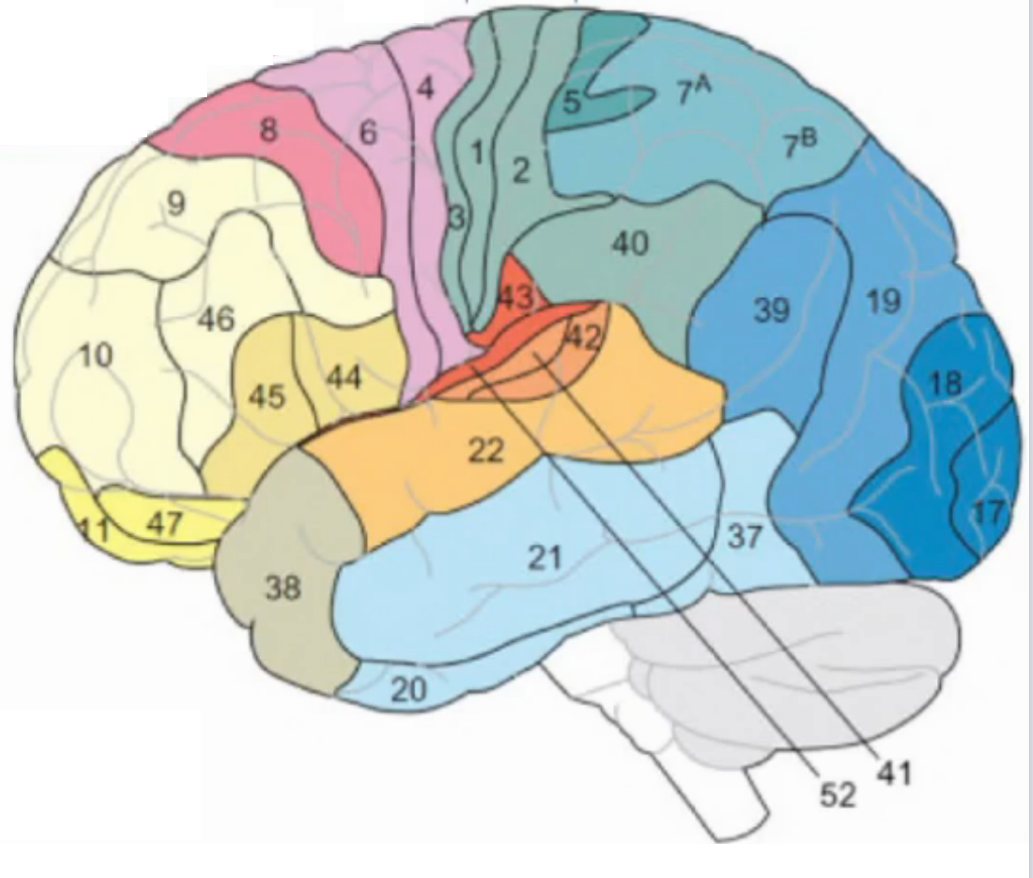
\includegraphics[width=0.8\textwidth]{cortex.png}
\end{center}



\end{column}

\pause

\begin{column}{6.5cm}

\begin{columns}[c]
\begin{column}{4cm}

\textbf{Hirnstamm}: Haltung, Gesichtsmuskulatur 


\end{column}

\begin{column}{2.5cm}


\begin{center}
    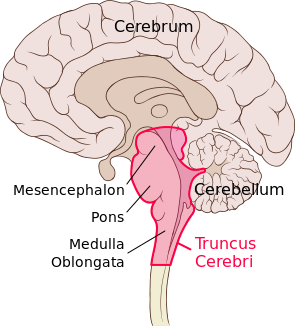
\includegraphics[width=0.8 \textwidth]{brain_stem.png}
\end{center}


\end{column}

\end{columns}

\pause

\begin{columns}[c]


\begin{column}{3cm}


\begin{center}
    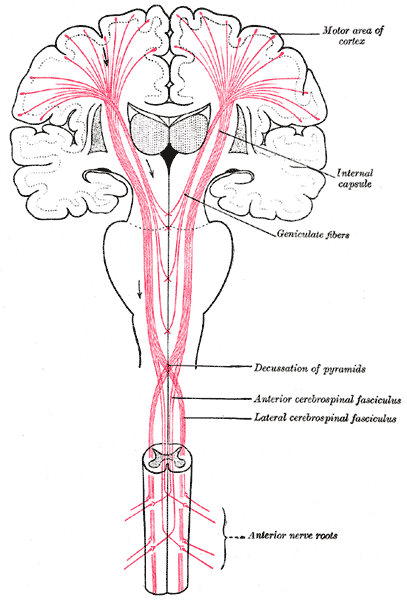
\includegraphics[width=\textwidth]{pyramidenbahn.png}
\end{center}
\end{column}


\begin{column}{3.5cm}



\textbf{Pyramidenbahn}: Axone aus dem Kortex (meist) über Interneurone zu \(\alpha\)-Motoneuronen. Afferenzen erlauben Feedback über Ist-Zustand.


\end{column}


\end{columns}


\end{column}






\end{columns}



\end{frame}


%% Pyramidenbahn? 967
\begin{frame}{IMPP Fragen}
    
\textbf{Welche Aussage zur Pyramidenbahn trifft zu?} \\[0.2 cm]

\begin{itemize}
\item[A.] Diejenigen Nervenfasern, die monosynaptisch an \(\alpha\)-Motoneuronen enden, sind überwiegend dünn myelinisiert (bis \(5\,\mu\) Durchmesser).
\item[B.] Etwa \(98\,\%\) der Axone enden im Rückenmark direkt an \(\alpha\)-Motoneuronen.
\item[C.] Ihre Neurone sind mehrheitlich dopaminerg.
\item[D.] Signale der Bahn erreichen über Axonkollateralen nach synaptischer Umschaltung das Kleinhirn. %% correct
\item[E.] Über diese Bahn laufende transkortikale Dehnungsreflexe (Long-Loop-Reflexe) haben typischerweise eine Reflexzeit von weniger als \(10\,ms\)

\end{itemize}    

\end{frame}


\begin{frame}{IMPP Fragen}
    
\textbf{Welche Aussage zur Pyramidenbahn trifft zu?} \\[0.2 cm]

\begin{itemize}
\item[A.] Diejenigen Nervenfasern, die monosynaptisch an \(\alpha\)-Motoneuronen enden, sind überwiegend dünn myelinisiert (bis \(5\,\mu\) Durchmesser).
\item[B.] Etwa \(98\,\%\) der Axone enden im Rückenmark direkt an \(\alpha\)-Motoneuronen.
\item[C.] Ihre Neurone sind mehrheitlich dopaminerg.
\item[D.] \textcolor{blue}{Signale der Bahn erreichen über Axonkollateralen nach synaptischer Umschaltung das Kleinhirn.}  \\ %% correct
\textcolor{blue}{\emph{Vergleich Ist-Zustand und Soll-Zustand durch untere Olive und Kleinhirn; ermöglicht Anpassung der Bewegung}}
\item[E.] Über diese Bahn laufende transkortikale Dehnungsreflexe (Long-Loop-Reflexe) haben typischerweise eine Reflexzeit von weniger als \(10\,ms\)

\end{itemize}    

\end{frame}



%% 178 - Parkinson Fall


\begin{frame}{IMPP Fragen}
    
\textbf{Ein 53-jähriger Lokomotivführer kommt mit einem seit 1 Jahr progredienten Ruhetremor an den Händen in die Hausarztpraxis. Die klinischen Untersuchungen ergeben eine körperliche Verlangsamung und ein kleinschrittiges Gangbild mit gebeugter Körperhaltung. Es wird die Indikation für eine medikamentöse Erstbehandlung gestellt. }

\textbf{Welche Wirkung ist therapeutisch am ehesten indiziert? Aktivierung von \dots } \\[0.2 cm]

\begin{itemize}
\item[A.] Dopaminrezeptoren im Coprus striatum %% correct
\item[B.] Dopaminrezeptoren im Ncl. dentatus 
\item[C.] GABA-Rezeptoren im Ncl. dentatus
\item[D.] Serotonin-Rezeptoren im Corpus striatum
\item[E.] Serotonin-Rezeptoren im Ncl. dentatus  

\end{itemize}    

\end{frame}



\begin{frame}{IMPP Fragen}
    
Ein 53-jähriger Lokomotivführer kommt mit einem seit 1 Jahr progredienten \textcolor{blue}{\textbf{Ruhetremor}} an den Händen in die Hausarztpraxis. Die klinischen Untersuchungen ergeben eine \textcolor{blue}{\textbf{körperliche Verlangsamung}} und ein \textcolor{blue}{\textbf{kleinschrittiges Gangbild}} mit gebeugter Körperhaltung. Es wird die Indikation für eine medikamentöse Erstbehandlung gestellt. 


\begin{itemize}
\item[A.] \textcolor{blue}{Dopaminrezeptoren im Coprus striatum} %% correct
\end{itemize}    

\begin{center}
    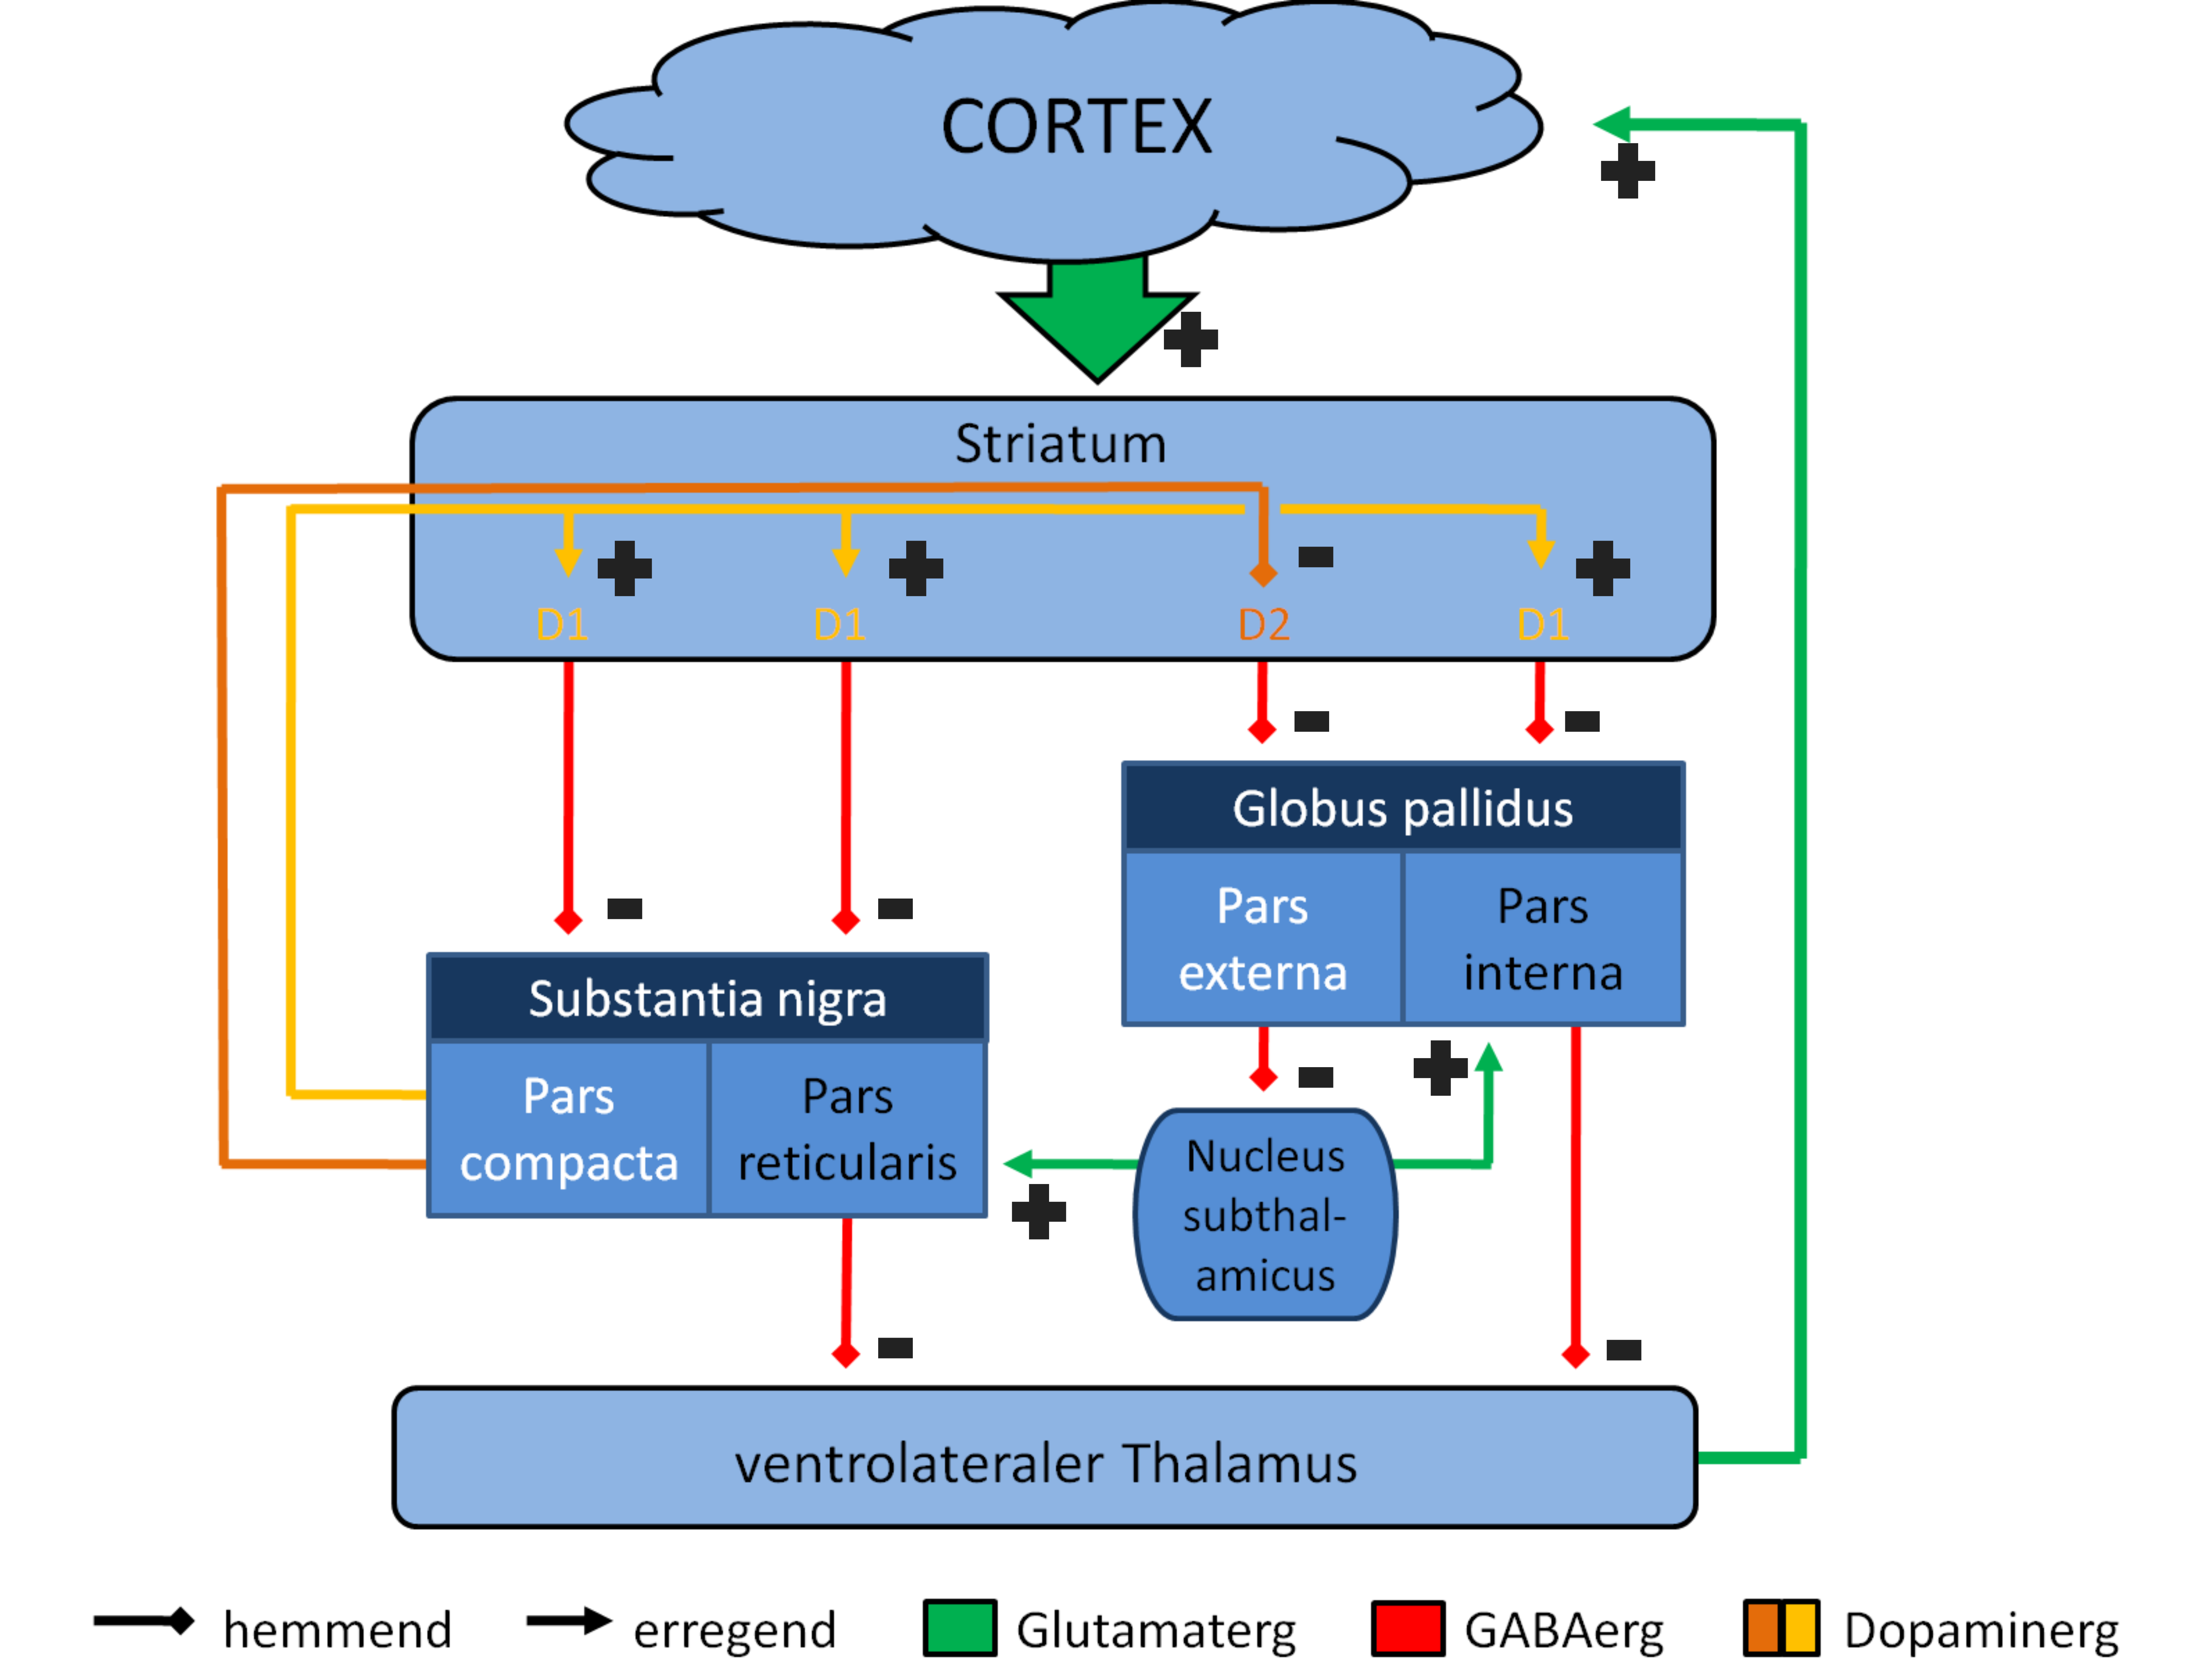
\includegraphics[width=0.6\textwidth]{Basalganglien_all.png}
    
\end{center}


\end{frame}







\end{document}
 
%%% Frequently used snippets

%% \begin{columns}[c]

%% \begin{column}{5cm}
%% \end{column}

%% \begin{column}{5cm}
%% \end{column}


%% \end{columns}




%% IMPP Frage

% \textbf{Frage} \\[0.2 cm]

% \begin{itemize}
% \item[A.]
% \item[B.]
% \item[C.]
% \item[D.]
% \item[E.]

% \end{itemize}